%%%%%%%%%%%%%%%%%%%%%%%%%%%%%%%%%%%%%%%%%%%%%%%%%%%%
% Document type, global settings, and packages
%%%%%%%%%%%%%%%%%%%%%%%%%%%%%%%%%%%%%%%%%%%%%%%%%%%%

\documentclass[12pt]{report}   %12 point font for Times New Roman
%Allows placement of graphics.
\usepackage[pdftex]{graphicx}
\DeclareGraphicsExtensions{.pdf}
\graphicspath{ {./figures/} }

\usepackage[letterpaper, left=1.2in, right=1in, top=1in, bottom=1in]{geometry}
\usepackage{setspace}  %use this package to set linespacing as desired
\usepackage{amsmath}
\usepackage{amsfonts}
\usepackage{amssymb}
%\usepackage{cite}
% \usepackage{times}  %set Times New Roman as the font
\usepackage[explicit]{titlesec}  %title control and formatting
\usepackage[titles]{tocloft}  %table of contents control and formatting
\usepackage[backend=bibtex, sorting=none, style=numeric-comp, bibstyle=ieee]{biblatex}  %reference manager
\usepackage[page]{appendix}  %for appendices
\usepackage{rotating}  %for rotated, landscape images
\usepackage[normalem]{ulem}  %for italicized text
\usepackage{listings} % for inline code
\usepackage{rotating} % for rotating the graphics 90 degrees

%% Define your title, your name, your school, and your month and year of graduation here
\newcommand{\thesisTitle}{Optimization Problems in Computational Physics: from Atoms to Molecular Assemblies}

\newcommand{\degreeType}{Dissertation}
\newcommand{\yourDegree}{Doctor of Philosophy}
\newcommand{\yourMajor}{Physics}
\newcommand{\yourName}{Christopher A. Mirabzadeh}
\newcommand{\yourSchool}{University of Idaho}
\newcommand{\majorprof}{F. Marty Ytreberg}
\newcommand{\memberone}{Andreas E. Vasdekis}
\newcommand{\membertwo}{Christine Berven}
\newcommand{\memberthree}{Jagdish Patel}
\newcommand{\deptAdmin}{Ray von Wandruszka}
\newcommand{\yourMonth}{August}
\newcommand{\yourYear}{2019}

% Define your quote and author for the epigraph here
\newcommand{\yourQuote}{
\textit{
        Without hope,without witness, without reward --River Song
    }
}

% Define your dedication statement here
\newcommand{\yourDedication}{
    To my parents, my wife, and my children.
}

%%%%%%%%%%%%%%%%%%%%%%%%%%%%%%%%%%%
% Bibliography
%%%%%%%%%%%%%%%%%%%%%%%%%%%%%%%%%%%

%Add your bibliography file here
\bibliography{references}

% prevent certain fields in references from printing in bibliography
\AtEveryBibitem{\clearfield{issn}}
\AtEveryBibitem{\clearlist{issn}}

\AtEveryBibitem{\clearfield{language}}
\AtEveryBibitem{\clearlist{language}}

\AtEveryBibitem{\clearfield{doi}}
\AtEveryBibitem{\clearlist{doi}}

\AtEveryBibitem{\clearfield{url}}
\AtEveryBibitem{\clearlist{url}}

\AtEveryBibitem{%
  \ifentrytype{online}
    {}
    {\clearfield{urlyear}\clearfield{urlmonth}\clearfield{urlday}}}

%%%%%%%%%%%%%%%%%%%%%%
% Start of Document
%%%%%%%%%%%%%%%%%%%%%%


% Clears plain-page pg# settings, relocates pg#'s @ top-right-corner.
\makeatletter
\renewcommand{\ps@plain}{
\renewcommand\@oddhead{\hfill\normalfont\textrm{\thepage}}
\renewcommand\@evenhead{}
\renewcommand\@oddfoot{}
\renewcommand\@evenfoot{}}

%Changes leading pg#'s to roman style
\renewcommand{\thepage}{\roman{page}}

%Changes default indenting in list of figures to 0 
\makeatletter
\renewcommand*\l@figure{\@dottedtocline{1}{0em}{2.3em}}% Default: 1.5em/2.3em
\let\l@table\l@figure
\makeatother

%Margins
% \addtolength{\voffset}{-.5in}
% \addtolength{\hoffset}{-.25in}
% \setlength{\marginparwidth}{1in}
% \setlength{\oddsidemargin}{.375in}
% \setlength{\marginparsep}{0in}
% \setlength{\topmargin}{12pt}
% \setlength{\headheight}{12pt}
% \setlength{\headsep}{20pt}
% \setlength{\textheight}{9in}
% \setlength{\textwidth}{6.5in}
% \setlength{\footskip}{0in}

\begin{document}

\onehalfspacing  %set line spacing

%Sets non-header pages numbering to same format (location) as header pages, e.g upper-right.
\pagestyle{myheadings}

%%%%%%%%%%%%%%%%%%%%%%%%%%%%%%%%%%%%%
% Title Page
%%%%%%%%%%%%%%%%%%%%%%%%%%%%%%%%%%%%%

%%%%%%%%%%%%%%%%%%%%%%%%%%%%%%%%%%%%%%%%%%%%%%%%%%%%%%%%%
% Do not edit these lines unless you wish to customize
% the template
%%%%%%%%%%%%%%%%%%%%%%%%%%%%%%%%%%%%%%%%%%%%%%%%%%%%%%%%%

\begin{titlepage}
\begin{center}
\vspace*{\fill} % vertical center

\thesisTitle\\
\vspace{3\baselineskip}
A \degreeType\\
Presented in Partial Fulfillment of the Requirements for the\\
Degree of \yourDegree\\
with a\\
Major in \yourMajor\\
in the\\
College of Graduate Studies\\
\yourSchool\\
by\\
\yourName\\
\vspace{5\baselineskip}
Major Professor: \majorprof, Ph.D.\\
Committee Members: 
\memberone, Ph.D.;
\membertwo, Ph.D.; \\
\memberthree, Ph.D.\\
Department Administrator: \deptAdmin, Ph. D.\\

\vspace{5\baselineskip}
\yourMonth{} \yourYear{}
\vfill
\vspace*{\fill}

\end{center}
\end{titlepage}
\clearpage

%%%%%%%%%%%%%%%%%%%%%%%%%%%%%%%%%%%%%
% Approval Page
%%%%%%%%%%%%%%%%%%%%%%%%%%%%%%%%%%%%%

%Authorization to Submit Thesis

%%%%%%%%%%%%%%%%%%%%%%%%%%%%%%%%%%%%%%%%%%%%%%%%%%%%%%%%%
% Do not edit these lines unless you wish to customize
% the template
%%%%%%%%%%%%%%%%%%%%%%%%%%%%%%%%%%%%%%%%%%%%%%%%%%%%%%%%%
\addcontentsline{toc}{chapter}{Authorization to Submit}
\section*{\large{Authorization to Submit \degreeType}}


\begin{flushleft}
This \MakeLowercase{\degreeType} of \yourName, submitted for the degree of \yourDegree \ with a major in \yourMajor \ and titled ``\thesisTitle," has been reviewed in final form. Permission, as indicated by the signatures and dates given below, is now granted to submit final copies to the College of Graduate Studies for approval.

\vspace{3\baselineskip}

\begin{tabular}{@{}lp{2.8in}lp{1.2in}@{}}

Major Professor: & \hrulefill & Date: &\hrulefill \\
                 & \majorprof, Ph.D. \\
                 \\
Committee Members: & \hrulefill & Date: &\hrulefill \\
                   & \memberone, Ph.D. \\
                   \\
                   & \hrulefill & Date: &\hrulefill \\
                   & \membertwo, Ph.D. \\
                   \\
                   & \hrulefill & Date: &\hrulefill \\
                   & \memberthree, Ph.D. \\
                   \\
Department \\ Administrator: & \hrulefill & Date: &\hrulefill \\
                          & \deptAdmin, Ph.D. \\
\end{tabular}
\end{flushleft}

\setcounter{page}{2} % set the page number appropriately
\clearpage

%%%%%%%%%%%%%%%%%%%%%%%%%%%%%%%%%%%%%
% Abstract
%%%%%%%%%%%%%%%%%%%%%%%%%%%%%%%%%%%%%

\addcontentsline{toc}{chapter}{Abstract}

\section*{\large{Abstract}}

\begin{flushleft}
% Insert your text here

Computer simulations are an invaluable tool in physics to help understand underlying mechanisms and explore parameter space without the need to perform costly experiments. This dissertation outlines two optimization problems in computational physics. The first is using molecular modeling to estimate the free energy---a fundamental physical quantity. The second is using finite element analysis to design a superconducting magnet system that could be used to efficiently store mechanical energy. As a measure of the amount of energy available to do work, the free energy is important for understanding, e.g., how amino acid mutations affect protein-protein interactions or when designing new drugs. Here, we present an implementation of the Monte Carlo adaptive integration method (AIM) in the popular molecular dynamics software package, GROMACS. We used AIM to calculate free energies in two model molecular systems and compared these results against a suite of standard methods. We showed that AIM converges with less simulation time than standard methods. We have also investigated the use of Halbach magnet arrays in combination with high-temperature superconductors for magnetic levitation of a fly-wheel energy storage system. Halbach arrays were selected because they have properties that are expected to be beneficial for efficient energy storage. To find the optimum orientation of the magnets for the arrays, we used Infolytica Magnet, a finite-element computation software package, to iterate over all permutations of magnet arrays consisting of 3 and 5 magnets in single and double layers. The fields and levitation forces as well as the width of the magnet arrays relative to the width of the superconductor were analyzed. We present our findings for the optimal array of this type and suggest guidelines to increase the levitation force of a superconducting magnetic bearing. 

\end{flushleft}
\clearpage

%%%%%%%%%%%%%%%%%%%%%%%%%%%%%%%%%%%%%
% Acknowledgments
%%%%%%%%%%%%%%%%%%%%%%%%%%%%%%%%%%%%%

% Acknowledgements are used to convey your appreciation to those who were instrumental to your academic career, including faculty, grant and scholarship agencies, internships, research facilities, and others who assisted and supported you along the way.

\addcontentsline{toc}{chapter}{Acknowledgements}
\section*{\large{Acknowledgements}}

\begin{flushleft}

%Insert your text here
The Graduate Physics program at the University of Idaho has given me the skills and
confidence that I need in order to accept new and interesting challenges. I would like to acknowledge the Ytreberg lab, it's members, and my committee members for all of their support over the years. Thank you.
Support for part of this research was provided by the National Science Foundation (DEB 1521049 and OIA 1736253) and the Center for Modeling Complex Interactions sponsored by the National Institutes of Health (P20 GM104420). Computer resources were provided in part by the Institute for Bioinformatics and Evolutionary Studies Computational Resources Core sponsored by the National Institutes of Health (P30 GM103324).
We would like to thank Infolytica Corporation for the use of their Finite Element Package, MagNet, and Dr. Gilles Fillion for his instructive and timely correspondence.  Funding for part of this research was provided by The NASA Ralph Steckler Space Grant.

\end{flushleft}
\clearpage

%%%%%%%%%%%%%%%%%%%%%%%%%%%%%%%%%%%%%
% Dedication
%%%%%%%%%%%%%%%%%%%%%%%%%%%%%%%%%%%%%

%%%%%%%%%%%%%%%%%%%%%%%%%%%%%%%%%%%%%%%%%%%%%%%%%%%%%%%%%%
% Do not edit these lines unless you wish to customize
% the template
%%%%%%%%%%%%%%%%%%%%%%%%%%%%%%%%%%%%%%%%%%%%%%%%%%%%%%%%%
\addcontentsline{toc}{chapter}{Dedication}

\begin{center}

\vspace*{\fill}
\textbf{Dedication}\\
\vspace{\baselineskip}
\yourQuote \\
\yourDedication\\
\vspace*{\fill}

\end{center}

%\clearpage

%%%%%%%%%%%%%%%%%%%%%%%%%%%%%%%%%%%%%
% Statement of Contribution
%%%%%%%%%%%%%%%%%%%%%%%%%%%%%%%%%%%%%

\addcontentsline{toc}{chapter}{Statement of Contribution}

\section*{\large{Statement of Contribution}}

\begin{flushleft}
% Insert your text here
Chapter 2: Christopher Mirabzadeh drafted the manuscript, performed the computational simulations, created all of the figures, and performed analysis in consultation with Marty Ytreberg.

Chapter 3: Christopher Mirabzadeh drafted the manuscript, performed the computational simulations, created most of the figures, performed analysis and processed the experimental data in consultation with Christine Berven and Joe Law. Chris Birkinbine contributed figures and assisted with measurements. Daniel Schneider designed and manufactured  experimental apparatus. 

Chapter 4: Christopher Mirabzadeh drafted the manuscript, performed the computational simulations, created most of the figures, and performed analysis in consultation with Marty Ytreberg.

\end{flushleft}
\clearpage

%%%%%%%%%%%%%%%%%%%%%%%%%%%%%%%%%%%%%
% Table of Contents
%%%%%%%%%%%%%%%%%%%%%%%%%%%%%%%%%%%%%

% Format for Table of Contents
% Adds required dots between sections and page numbers in TOC
\renewcommand{\cftsecleader}{\cftdotfill{\cftsecdotsep}}
\renewcommand\cftsecdotsep{\cftdot}
\renewcommand\cftsubsecdotsep{\cftdot}
\renewcommand{\cftpartleader}{\cftdotfill{\cftdot}} % for parts
\renewcommand{\cftchapleader}{\cftdotfill{\cftdot}} % for chapters


% Names list of figures and table of contents explicitly and sets spacing above and below titles
\renewcommand{\listfigurename}{\vspace{-2.2cm} \large List of Figures \vspace{-1cm}}
\renewcommand{\listtablename}{\vspace{-2.2cm} \large List of Tables \vspace{-1cm}}
\renewcommand{\contentsname}{\vspace{-2.2cm} \large Table of Contents \vspace{-1cm}}
\addcontentsline{toc}{chapter}{Table of Contents}

\begin{singlespace}
\tableofcontents
\end{singlespace}

\clearpage

%%%%%%%%%%%%%%%%%%%%%%%%%%%%%%%%%%%%%
% List of figures and tables
%%%%%%%%%%%%%%%%%%%%%%%%%%%%%%%%%%%%%

\addcontentsline{toc}{chapter}{List of Tables}
\begin{singlespace}
	\setlength\cftbeforetabskip{\baselineskip}  %manually set spacing between entries
	\listoftables
\end{singlespace}

\clearpage

\addcontentsline{toc}{chapter}{List of Figures}
\begin{singlespace}
    \setlength\cftbeforefigskip{\baselineskip}  %manually set spacing between entries
    \listoffigures
\end{singlespace}

\clearpage

%%%%%%%%%%%%%%%%%%%%%%%%%%%%
%
% Chapters
%
%%%%%%%%%%%%%%%%%%%%%%%%%%%%

%%%%%%%%%%%%%%%%%%%%%%
% formatting
%%%%%%%%%%%%%%%%%%%%%%

% resume page numbering for rest of document
\clearpage
\pagenumbering{arabic}
\setcounter{page}{1} % set the page number appropriately

% Adjust chapter title formatting
\titleformat{\chapter}[display]
{\normalfont\bfseries}{\MakeUppercase\chaptertitlename\ \thechapter}{0pt}{\MakeUppercase{#1}}  %spacing between titles
\titlespacing*{\chapter}
  {0pt}{0pt}{30pt}	%controls vertical margins on title
  
% Adjust section title formatting
\titleformat{\section}{\normalfont\bfseries}{\thesection}{1em}{#1}

% Adjust subsection title formatting
\titleformat{\subsection}{\normalfont}{{\thesubsection}}{0em}{{\hspace{1em}#1}}

% Adjust subsubsection title formatting
\titleformat{\subsubsection}{\normalfont\itshape}{\thesubsection}{1em}{#1}
%%%%%%%%%%%%%%%%
% Introduction
%%%%%%%%%%%%%%%%

% \clearpage
% \section*{INTRODUCTION}
% \addcontentsline{toc}{chapter}{Introduction}
\chapter{Introduction}

Computer simulations allow us to explore ``what if'' situations by building a representative model that contains many of the parameters of the actual physical system, but in a virtual form. In this way, costly, time-consuming, or unsafe physical experiments may be avoided and, instead cheap and efficient in-silica ``experiments'' may be performed. Simulations can be used to develop a deeper understanding of a system and can support experiments by generating hypotheses or finding optimal values for input variables.

The goal of many simulations is to evaluate the effect of changing variables in a system, often to determine optimal values. A key advantage to simulation over experiment is the ability to capitalize on existing mathematical and computational techniques to determine optimal values without the need to test every possible value.

Another benefit to simulations is their ability to simulate non-physical processes. For example, in Chapter 2 below we enhance the speed of a simulation by giving atoms non-physical properties. According to the laws of statistical mechanics the final results are physically relevant, even though the intermediate steps are not.

The topic of the first part of this dissertation is free energy calculation in molecular systems. The free energy is a fundamental physical quantity that determines whether a system will spontaneously change between states, and more specifically, gives the relative amount of time a system will spend in each state. Estimating the free energy for molecular system is a powerful tool, e.g., to determine how amino acid mutations modify protein folding or binding, or for developing new drugs. A long-standing goal of our research group is to develop and test methods for efficient free energy computation. In Chapter 2 we have implemented the previously-developed adaptive integration method (AIM) in a popular molecular modeling software package. We tested our implementation on two molecular systems and show that our results converge to a higher level of accuracy and precision for a given simulation time as compared to standard methods.

The molecular modeling used in Chapter 2 moves all the atoms in the system by calculating interactions at the atomic level. While this is a valuable approach for studying small molecular systems it is not useful for studying large-scale systems such as mechanical stress on an engine. Thus, in Chapter 3 we used the finite element method where the surface of any physical object is broken into a mesh of smaller parts called finite elements. Forces between objects are then approximated by summing the forces for all elements. Smaller elements provide greater accuracy and allow us to represent more complex geometries.

The purpose of the research in Chapter 3 is to examine the force configurations of alternating arrangements of permanent magnet arrays, called Halbach arrays. The ultimate goals is to design a superconducting flywheel energy storage system for use in deep space. For this study we used two-dimensional finite element analysis in order to determine the optimal configuration for our permanent magnet arrays. These simulations allowed us to find the optimum configuration of magnets by exploring every possible magnet configuration in a matter of hours instead of spending months in a lab. 


%%%%%%%%%%%%%%%%
% Chapter 2
%%%%%%%%%%%%%%%%

\chapter{Implementation of Adaptive Integration Method for Free Energy Calculations in Molecular Systems}
CA Mirabzadeh, F. Marty Ytreberg

\begin{center}
    To be submitted in \textit{PeerJ} — the Journal of Life and Environmental Sciences
\end{center}

\section*{Abstract}
Estimating free energy differences by computer simulation is useful for a wide variety of applications such as creating drug designs and for understanding how amino-acid mutations modify protein interactions. However, calculating free energy differences remains challenging and often requires extensive trial and error and very long simulation times in order to achieve converged results. Here, we present an implementation of the adaptive integration method (AIM) that was tested on two molecular systems and validated by comparing results from AIM to those from a suite of standard methods. The model systems tested here include calculating the solvation free energy of methane, and the free energy of mutating the peptide GAG to GVG. We show that AIM is more efficient than standard methods for these test cases, that is, AIM results converge to a higher level of accuracy and precision for a given simulation time.

\section{Introduction}

Measuring free energy differences using computer simulations can be computationally expensive, yet is useful for many different applications (see e.g., \cite{Mobley2013,Zhan2013,Zhan2015,Wichman2016,Chodera2011a, SteinBrecher2010, Cournia2017, Miller2014, Petukh2015}) such as determining protein conformational preferences or for virtual screening in drug design \cite{Zhan2015, SteinBrecher2010, Chodera2011a}. Of specific relevance to the current study is that free energy calculations allow for prediction of how amino acid mutations will modify protein-protein binding \cite{Wichman2016, Zhan2013, Miller2014, Petukh2015}. We are particularly interested in developing and implementing efficient methods for calculating free energy differences and using them to understand protein evolution and protein-protein binding. 

For this report, we have implemented the adaptive integration method (AIM), introduced by Fashnacht et al. \cite{Fasnacht2004}, for use in the GROMACS \cite{Berendsen1995} molecular dynamics simulation package. Though there are many free energy methods for molecular systems (see e.g., \cite{Kofke2005,Goncalves2004,Lyubartsev1996, Shirts2007,Klimovich2015,Chodera2011}), in previous studies AIM has shown promise to provide high quality, precise and efficient estimates of binding free energies\cite{Ytreberg2006}. AIM is an adaptive sampling method that continuously improves the estimate for free energy during the simulation.  AIM uses Monte Carlo to randomly sample $\lambda$ space in order to obtain numerical estimates of the free energy differences. The algorithm actively ``learns'' points of high variation along the reaction pathway and increases sampling in those areas.

For comparison with other free energy methods we used the Python tool, alchemical-analysis.py \cite{Klimovich2015}, which is part of the Pymbar \cite{Shirts2008} package. The alchemical-analysis tool takes the output from molecular dynamics simulations and estimates the free energy using many different methods, including the Bennett acceptance ratio (BAR), multistate Bennett acceptance ratio (MBAR), thermodynamic integration (TI) and exponential averaging (IEXP, DEXP). Exponential averaging is known to be noisy, biased and dependent on the tails of the distribution of $\lambda$ states \cite{Bruckner2011,Shirts2005}. Bennett acceptance ratio and multistate Bennett acceptance ratio have been shown to be exceptionally accurate with less $\lambda$ states required\cite{Shirts2005}. Thermodynamic integration can be biased by the chosen method of integration. Some of that bias can be removed by using cubic-spline interpolation or more complex integration estimators\cite{Shirts2005, Shyu2009}.

For the current study we chose two molecular systems that have well-documented results and are important starting points for biomolecular free energy studies. First, we calculated the solvation free energy of methane. Simulations were performed and the free energies were calculated using the standard methods provided by alchemical-analysis. Simulations were also performed using AIM and results compared to standard simulations. Once we were confident in our results and our strategy, we calculated the free energy of mutating GAG to GVG in water. For both systems, we found that AIM produces free energy estimates that are within statistical uncertainty of standard methods but with greater efficiency (i.e., more accurate for a given simulation time).

\section{Methods}

For this study we performed alchemical free energy simulations where the system is changed from a reference state to an end state by constructing a reaction pathway that either adds or removes a small molecule of interest. Such alchemical simulations are non-physical, thus the simulation does not represent what would occur naturally. Since the free energy is a state variable, it is independent of the path taken, and we are free to provide any path we wish. To perform these simulations the reaction pathway is divided into many separate, non-physical, $\lambda$ states between a reference state and an end state. The $\lambda$ states represent the progression along a reaction pathway as the reference state transforms into the end state. 

Like most methods used to calculate free energies we start from the free energy identity,

\begin{equation}\label{eq:free_id}
    F = U - TS
\end{equation}

Where $U$ is the potential energy, $T$ is the temperature and $S$ is the entropy of the system.

For free energy differences we generalize the formulation of the change in free energy by separating calculations into two, non-overlapping, thermodynamic end states, $A$ and $B$, at constant temperature $T$,

\begin{equation}
    \Delta F_{A \rightarrow B} = F_{B} - F_{A}= \Delta U - T \Delta S
\end{equation}

Where $\Delta F$ is the change in free energy, $\Delta U$ is the change in potential energy and $\Delta S$ is the change in entropy of the system.

Derived from statistical mechanics, the free energy difference between the two end states, A and B, of the system is the log of the ratio of probabilities related to the energy states, $U_{A}(\vec{x})$ and $U_{B}(\vec{x})$,

\begin{equation}\label{eq:free}
    \Delta F = -k_{B}T \ln{\frac{Z[U_{B}(\vec{x})]}{Z[U_{A}(\vec{x})]}}
\end{equation}

Where $k_{B}$ is the Boltzmann constant, T is the system temperature. $Z[U(\vec{x})]$ is the partition function for the energy states, $U_{A}(\vec{x})$ and $U_{B}(\vec{x})$, where $\vec{x}$ is the vector of configuration coordinates,

\begin{equation}\label{eq:part}
    Z[U(\vec{x})] = \int dx \exp{(-\beta U(\vec{x})})
\end{equation}

Here we have substituted $\beta = \frac{1}{k_{B}T}$. Computationally, we calculate free energy differences between end states by sampling molecular dynamics simulations along a reaction pathway of intermediate states, defined by $\lambda$, such that,

\begin{equation}
    0 \leq \lambda \leq 1
\end{equation}

This pathway connects the two end states of the system. In the case of poor overlap, where the end states may be separated by a high energy barrier, $|U_{B} - U_{A}| \gg k_{B}T$, this pathway mitigates the otherwise very slow convergence of free energy estimates \cite{Shirts2007}. Care should be taken when choosing intermediate states such that there is adequate overlap in the conformation space between the end states \cite{Shirts2007, Klimovich2015}. For our simulations the number of $\lambda$'s and time per $\lambda$ were chosen through extensive trial and error. 

For the standard methods we ran fixed $\lambda$ alchemical simulations. During alchemical simulations we first take a molecular dynamics step, where we calculate the inter-atomic forces and other states of the system. We then take a step in $\lambda$ space where we can apply transformations against the system state. Fixed $\lambda$ simulations spend a fixed amount of time at each intermediate $\lambda$ state. For AIM the amount of time at each intermediate $\lambda$ state is decided by the algorithm.

With proper intermediate states, we are now able to use a method, such as thermodynamic integration (TI), to calculate the free energy difference between the two end states. For thermodynamic integration we are simply taking the derivative of Eq.\ \ref{eq:free_id} with respect to $\lambda$,

\begin{equation}\label{eq:diffeq}
    \frac{\partial F}{\partial \lambda} = \left< \frac{\partial U}{\partial \lambda} \right>_{NVT}
\end{equation}

This differential equation, Eq.\ \ref{eq:diffeq}, can then be integrated to give us,

\begin{equation}\label{eq:ti}
    \Delta F = \int_{\lambda = 0}^{1} \left< \frac{\partial U_{\lambda}(\vec{x})}{\partial \lambda} \right>_{\lambda} d\lambda
\end{equation}

Where the $\langle \cdot \rangle_{\lambda}$ notation represents the ensemble average at a given intermediate state, $\lambda$. We are then free to estimate the free energy by integrating Eq.\ \ref{eq:ti} after running equilibrium simulations at each intermediate $\lambda$ state.

The method of exponential averaging \cite{Zwanzig1954} starts from Eq.\ \ref{eq:free} above and then adding and subtracting $\exp{(-\beta U(\vec{x}))}$ from the integral in the partition function of the numerator we end up with the final relationship,

\begin{equation}\label{eq:exp}
    \Delta F = -k_{B}T \ln \langle \exp{(-\beta U(\vec{x}))} \rangle
\end{equation}

Unlike most other methods, exponential averaging has an exact solution since it is only used to evaluate the difference between two states. However, it is the least efficient method and should not be used if difference in potential energies are much larger than $k_{B}T$ \cite{Shirts2005}.

The Bennett \cite{Bennett1976} and multistate \cite{Shirts2008} Bennett acceptance ratio (BAR and MBAR) methods are far more efficient than exponential averaging and are perhaps the most efficient of the current standard free energy methods \cite{Shirts2005, Ytreberg2006}. BAR and MBAR typically achieve the same statistical precision as TI with fewer $\lambda$ states unless the integrand for TI is very smooth \cite{Monticelli2013, Ytreberg2006}. The complete derivation can be found in Bennett's paper \cite{Bennett1976} but the premise is; for sufficiently large samples $n_{i}$ of $U_{i}$ and $n_{j}$ of $U_{j}$,

\begin{equation}\label{eq:bar}
    \Delta F(i \rightarrow j) = k_{B}T \ln{\frac{\langle f(\Delta U_{ij} + C) \rangle_{j}}{\langle f(\Delta U_{ji} - C) \rangle_{i}}} + C 
\end{equation}

where C is a shift constant:

\begin{equation}\label{eq:barc}
    C = k_{B}T\ln{\frac{n_{j}}{n_{i}}}
\end{equation} 

and $f(x)$ is the Fermi function:

\begin{equation}\label{eq:fermi}
    f(x) = \frac{1}{1 + \exp{\beta x}} 
\end{equation}

Equation\ (\ref{eq:bar}) is the ratio of canonical averages of two different potentials $U_{i}$ and $U_{j}$ acting on the same configuration space meaning it requires information from two neighboring states. However, this limitation is not too much of a concern with a trivial coordinate transformation or when using dummy coordinates in alchemical simulations. MBAR, an extension of BAR, differs in that it takes data from more than two states hence the name "multistate".

AIM looks to solve the same equation as thermodynamic integration (Eq.\ \ref{eq:ti}) with the exception that we are performing the approximation during the simulation as opposed to after. As a Monte Carlo method of the Metropolis form we move from state $\lambda_{old}$ to $\lambda_{new}$ with an acceptance probability

\begin{equation}\label{eq:aimaccept}
\min\{1,\exp(- \beta( U_{new} - U_{old})+\beta(F_{new} - F_{old})\}
\end{equation}

where $U_{new} - U_{old}$ is the difference in the potential energy for the old and new $\lambda$ values and $F_{new} - F_{old}$ is the current approximate for the free energy based on the running average of the $\frac{dU}{d\lambda}$ terms. AIM thus involves an independent trial move (including generation of the random number) for reaction coordinate space ($\lambda$ for our study) vs configuration space.

\subsection{Implementation}

AIM was implemented into GROMACS as an expanded ensemble calculation; the Hamiltonian must be calculated along with its derivative, and an expanded ensemble step must be performed for every dynamics step. In GROMACS, \texttt{nstexpanded} is the number of integration steps between attempted $\lambda$ moves changing the system Hamiltonian in expanded ensemble simulations. This value must be a multiple of \texttt{nstcalcenergy}, the number of steps before calculating the system energy, but can be greater or less than \texttt{nstdhdl}, the number of steps before calculating dHd$\lambda$. For a detailed explanation of all technical terms see: \cite{gmxmanual}. See the appendix for a direct example in usage.

AIM requires the dHd$\lambda$ value from every dynamics step to be stored regardless of whether a move in $\lambda$ space is attempted. Since dHd$\lambda$ is only calculated at each step where free energies are calculated, every \texttt{nstdhdl} step, we set \texttt{nstexpanded} = \texttt{nstdhdl} = \texttt{nstcalcenergy} = 1 for AIM simulations. This further implies that \texttt{lmc-stats} functions were not used during AIM simulations because those functions modify the Hamiltonian which is counter intuitive for AIM as the algorithm requires the derivative of the unmodified Hamiltonian. Making a comparison between a modified Hamiltonian and its unmodified derivative would require re-weighting which introduces statistical noise and is entirely impractical.

For the implementation of AIM with GROMACS we follow the outline given in our previous study \cite{Ytreberg2006}. 
\begin{enumerate}
\item Start the simulation from an equilibrated configuration at $\lambda$=0 and perform one dynamics step. 
\item Use the Metropolis Monte Carlo sampler to choose the trial move, $\pm$ 1, in $\lambda$ space. If our $\lambda$ spacing is 0.05, a move from $\lambda$=0.35 to 0.4 or 0.3 may be attempted but not to 0.45. 
\item Calculate the difference in potential energy between $\lambda$ trial and $\lambda$ current.
\item Using the trapezoidal rule, we calculate the free energy difference between the running average of $\lambda$ trial and the running average $\lambda$ current. 
\item Attempt a Monte Carlo move in $\lambda$ space with acceptance probability given in Eq.\ \ref{eq:aimaccept}.
\item If the move is accepted then $\lambda$ is updated to the trial value, otherwise the simulations stays at current $\lambda$.
\item The running average of the free energy at $\lambda$ is updated.
\end{enumerate}

The final step updates the average of the free energy at $\lambda$, regardless of acceptance. This is done because the running average will continue to change since each consecutive approximation is independent of the previous. The running average improves the smoothness of the underlying free energy at $\lambda$ which may be from high/low energy regions that were poorly approximated before. Thus, whenever a better approximation of the probability distribution is needed, AIM generates new approximations that targets it. 

\subsection{Simulation Details}

All simulations described in this paper were performed using the molecular dynamics package GROMACS 5.1.4. The simulations were carried out at 300 K and solvated in a dodecahedron box with TIP3P waters. The molecule was parameterized using the OPLS (Optimized Potential for Liquid Simulations) force field \cite{Jorgensen1996}. The OPLS force field was chosen for this study because it is known to perform well on small molecules \cite{Shirts2003}. In future studies, we anticipate using AIM on protein systems where other force fields are more appropriate such as AMBER \cite{Salomon-Ferrer2013} and CHARMM \cite{Mackerell2001}. Since all MD force fields have similar form and number of parameters, it is expected that the performance of AIM would not depend on the force field chosen. 

For the GAG to GVG mutations, NaCl ions were added to keep the simulation box neutral and reach a physiologically relevant 150 mM salt concentration. Energy minimization was performed using steepest descent with 1000 steps. The system was then equilibrated using simulated annealing for 1000 ps to heat the system from 100K to 300K. For production simulations, electrostatic interactions were handled by Reaction field with a cut-off of 0.9 nm, Potential-shift-Verlet modifier and Verlet cutoff scheme. Van der Waals interactions were handled by twin range cut-offs with neighbor list cut-off of 1.15 nm and VdW cut-off 0.9 nm. The hydrogen bonds were constrained with the Shake algorithm, allowing for a longer time step of 2 fs. Long range dispersion corrections for energy and pressure were applied. 

In order to determine the best distribution of intermediate states we followed a simple strategy:
\begin{enumerate}
\item Conduct short simulations with a small set of intermediates
\item Generate a plot comparing slope values between AIM and fixed $\lambda$.
\item Determine the locations of curvature in the estimate of the free energy
\item Increase the density of intermediate states in locations of high curvature
\item Repeat until areas of high curvature have been well explored
\end{enumerate}

\section{Methane and GAG to GVG Solvation Free Energy}

The first system used here, methane in water, is detailed in a systematic study of force fields and the free energies of hydration of amino acid side chain analogs \cite{Sun1992,Lyubartsev1996,Chodera2011,Paliwal2011}.

For the GAG to GVG mutation the PMX \cite{Gapsys2015} software package was used to construct the tri-peptide mutation. Using the PMX web server (http://pmx.mpibpc.mpg.de), we generated the hybrid protein structure and topology for simulations of the chosen mutation, alanine to valine.

For each system, we calculated the free energy for decoupling the Lennard-Jones interactions between the atomic sites of the molecule of interest in water. For fixed $\lambda$ simulations, separate equilibrium simulations of equal length were run in order to represent each of the intermediate $\lambda$ states. The same values for $\lambda$ were used in both fixed $\lambda$ and AIM expanded ensemble simulations. The GROMACS package was altered to print out the dHd$\lambda$ averages computed by AIM to the log file when AIM is used as the \texttt{lmc-mover}. For fixed $\lambda$ simulations the free energy was estimated using an external tool, alchemical-analysis.py. AIM estimates were calculated using both the trapezoidal rule and cubic-spline. All methods and code may be made available upon request.

\section{Results}

\subsection{Methane}

After conducting short simulations, generating plots to determine locations of high curvature and increasing $\lambda$ density in those locations, we averaged eight trial simulations of 100 ps per $\lambda$ for separate $\lambda$ distributions, Fig.\ \ref{increasinglambdas}. We found, by progressively increasing the $\lambda$ density between $\lambda$ = 0.5 and $\lambda$ = 1.0, that a distribution of 31 $\lambda$s gave us a dense enough distribution to properly compare AIM to fixed $\lambda$ methods for the methane simulations.

Fig.\ \ref{methane31} is a violin plot used to visualize the distribution and probability density over the average of eight trials for each method versus time per $\lambda$. A violin plot combines a box plot and a density plot to show the shape of the distribution around the mean. The thick black bar in the center represents the interquartile range, the white dot is the median and the thin black line going vertically through the middle represents the upper and lower adjacent values. Reading a violin plot is similar to reading a density plot. The thicker parts represent high frequency values and the thinner parts represent low frequency values. The advantage of a violin plot over a box plot is that we are able to view the number of groupings in the underlying distribution of the data.

In Fig.\ \ref{methane31}, for 31 $\lambda$ values at 100 ps per $\lambda$, the slower convergence of MBAR leads to two separate distributions of converging points. At 500 ps the other methods are beginning to show signs of convergence, however, we see that AIM is forming a second distribution and the width of the distribution of the other methods has not condensed or flattened along the horizontal axis, suggesting convergence has not yet occurred for any of the methods. Despite this, the average of the methods are in agreement within uncertainty, i.e. variance in the mean of the estimated free energy. At 1 ns per $\lambda$ all methods are similarly converged, indicating the larger sample size has reduced the variance from the mean. 

\subsection{GAG to GVG Mutation}

For the GAG to GVG mutation we first tested a distribution of 41 $\lambda$ values averaged over 8 trial simulations of 1 ps and 100 ps per $\lambda$; see Fig.\ \ref{a2vlineplot}. By reviewing the smoothness of the function we concluded that 41 $\lambda$ values was sufficient and continued the simulations for 1 ns per $\lambda$. Fig.\ \ref{a2vviolinplot} shows distribution of the convergence over time for each method. We see that AIM has mostly converged at 100 ps per $\lambda$ and all methods have similarly converged for 1 ns per $\lambda$.

\section{Discussion}

In the limit of infinite sampling, all rigorous methods (i.e., statistically-mechanically-based methods), performed properly with the same force field and parameters, will yield the same result within uncertainty. For fixed $\lambda$ simulations the sampling time is typically chosen to be the same for each $\lambda$ state. Thus, we are led to increase sampling time whenever convergence has not been achieved. However, if bias is introduced by an insufficient $\lambda$ distribution, in areas of high variation, increased sampling leads to radical convergence problems \cite{Shyu2009, SteinBrecher2010}. If the curvature of the underlying free energy function is large, averaging over a state space that is not dense enough to fully describe the state function propagates this bias requiring significantly increased sampling time to achieve convergence. Increasing sampling time may not be realistic when dealing with limited computational resources. Paliwal et al. \cite{Paliwal2011} make a detailed argument to why convergence may not be possible for all systems due to hard limitations in computational resources. 

In particular, both TI and AIM are calculating the same slope averages and should agree very well for simple systems and reasonably long simulation times. However, due to the fact that AIM spends more time in regions of high variation, we should not expect the approximation of AIM to exactly match TI with similar sampling time until the $\lambda$ density, the number of intermediate states, has been sufficiently increased in high variance regions. Once we have chosen a sufficiently dense $\lambda$ space, reasonably long simulations should lead to highly similar approximations between these two methods.

Since AIM is implemented as a Metropolis Monte Carlo \cite{Metropolis1953} expanded ensemble \cite{Lyubartsev1996} method, where the approximation of a given intermediate state is adaptively expanded whenever a better approximation of the state is needed, AIM has improved sampling over fixed $\lambda$ simulations. AIM is able to smooth the underlying free energy function by spending more time at critical points in the curvature of the Hamiltonian state space. This means that AIM requires fewer $\lambda$ states to fully explore the free energy of a system because we minimize the overall variance of the free energy estimate by adjusting the distribution of data points in each intermediate $\lambda$ state based on the acceptance criteria. This reduces the propagation of error in poorly chosen, stationary distributions. 

The observant reader may note that AIM violates detailed balance, however, AIM does obey detailed balance asymptotically, i.e., once the free energy differences have converged. As simulation time increases to infinity the average free energy differences between states reach an equilibrium. 

\section{Conclusion}

In this report we have implemented the adaptive integration method (AIM) for calculating free energy differences in GROMACS and applied it to two molecular systems. We have shown agreement within statistical uncertainty between AIM and a suite of standard fixed $\lambda$ methods for methane solvation and an GAG to GVG mutation. We have also shown that AIM is more efficient than the other tested methods. That is, for a given amount of simulation time, AIM has a higher level of accuracy and precision compared to other methods.

Further, we found that running longer simulations with too few intermediate $\lambda$ states generated results that were inconsistent between methods. The density and sampling convergence of the $\lambda$ states directly influences the agreement between all the tested methods. Since some states will contribute disproportionately to the variance of the estimate, we found that testing short simulations of different $\lambda$ densities before attempting longer simulations is a more economical use of time and resources. In particular, we found that increasing the number of intermediate $\lambda$ values between 0.5 and 1.0 allows the free energy to become independent of the number of values which allows AIM and fixed $\lambda$ results to agree within statistical uncertainty for all systems that were tested.

\section{Acknowledgments}
Support for this research was provided by the National Science Foundation (DEB 1521049 and OIA 1736253) and the Center for Modeling Complex Interactions sponsored by the National Institutes of Health (P20 GM104420). Computer resources were provided in part by the Institute for Bioinformatics and Evolutionary Studies Computational Resources Core sponsored by the National Institutes of Health (P30 GM103324).


\pagebreak

\begin{sidewaysfigure*}[htbp]
    \centering
    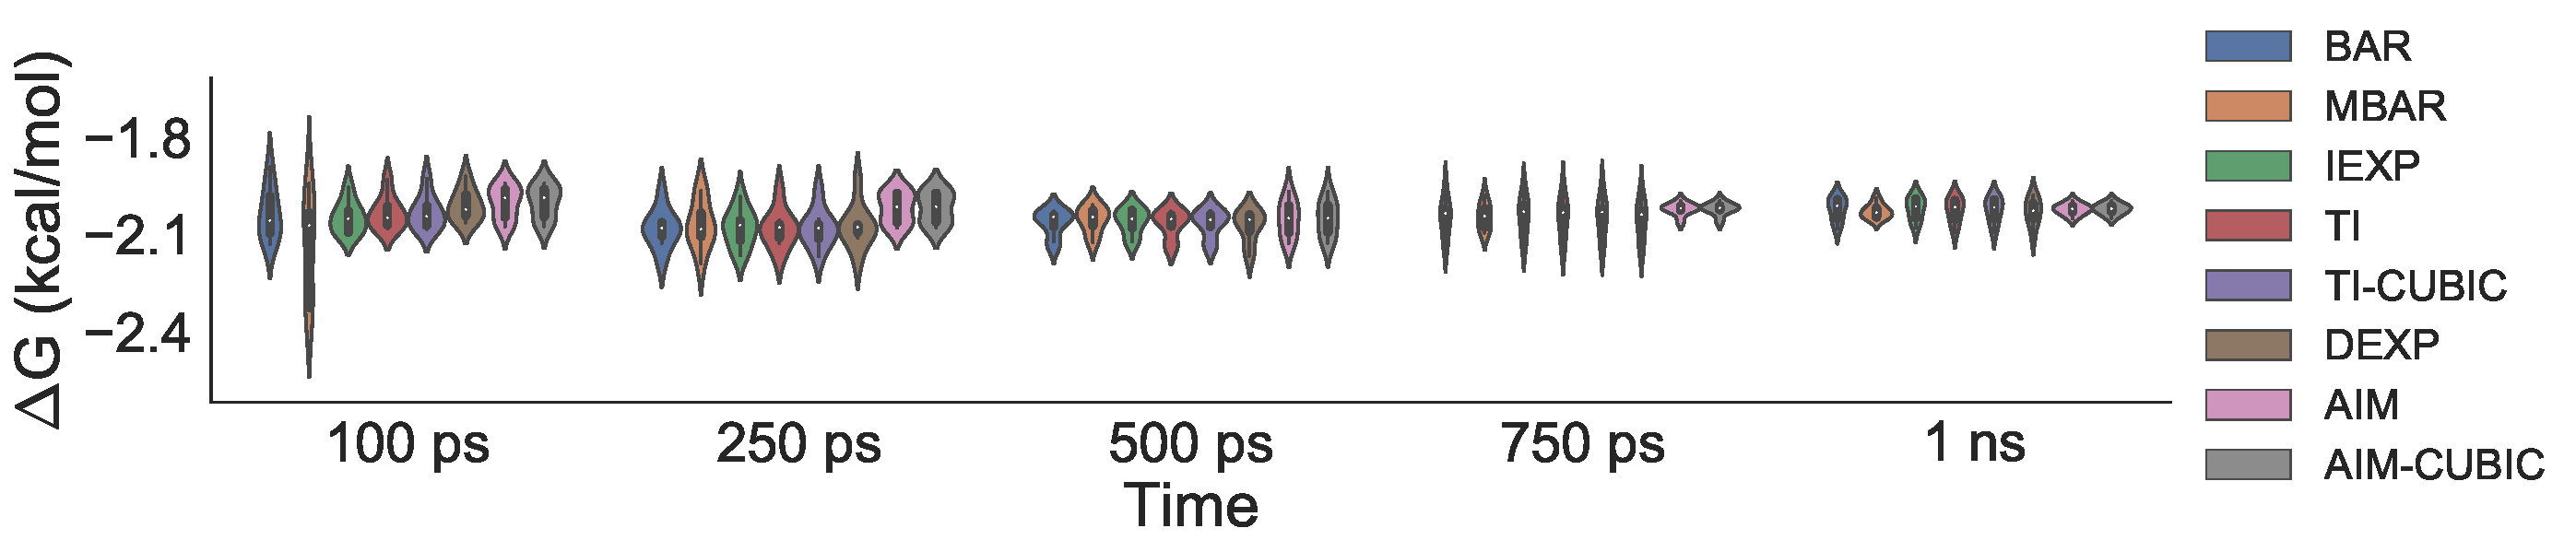
\includegraphics[width=1\textwidth]{Methane_31L_violinplotovertime}
    \caption{Violin plot showing methane solvation results for 31 $\lambda$ values averaged over eight trials. A violin plot combines a box plot and a density plot to visualize the distribution and probability density. The graphic shows all methods have similarly converged at 1 ns per $\lambda$ for the same number of intermediate states and sample size with AIM and AIM-CUBIC showing early convergence at 750 ps per $\lambda$.}
    \label{methane31}
\end{sidewaysfigure*}
\pagebreak


\begin{figure*}[htbp]
    \centering
    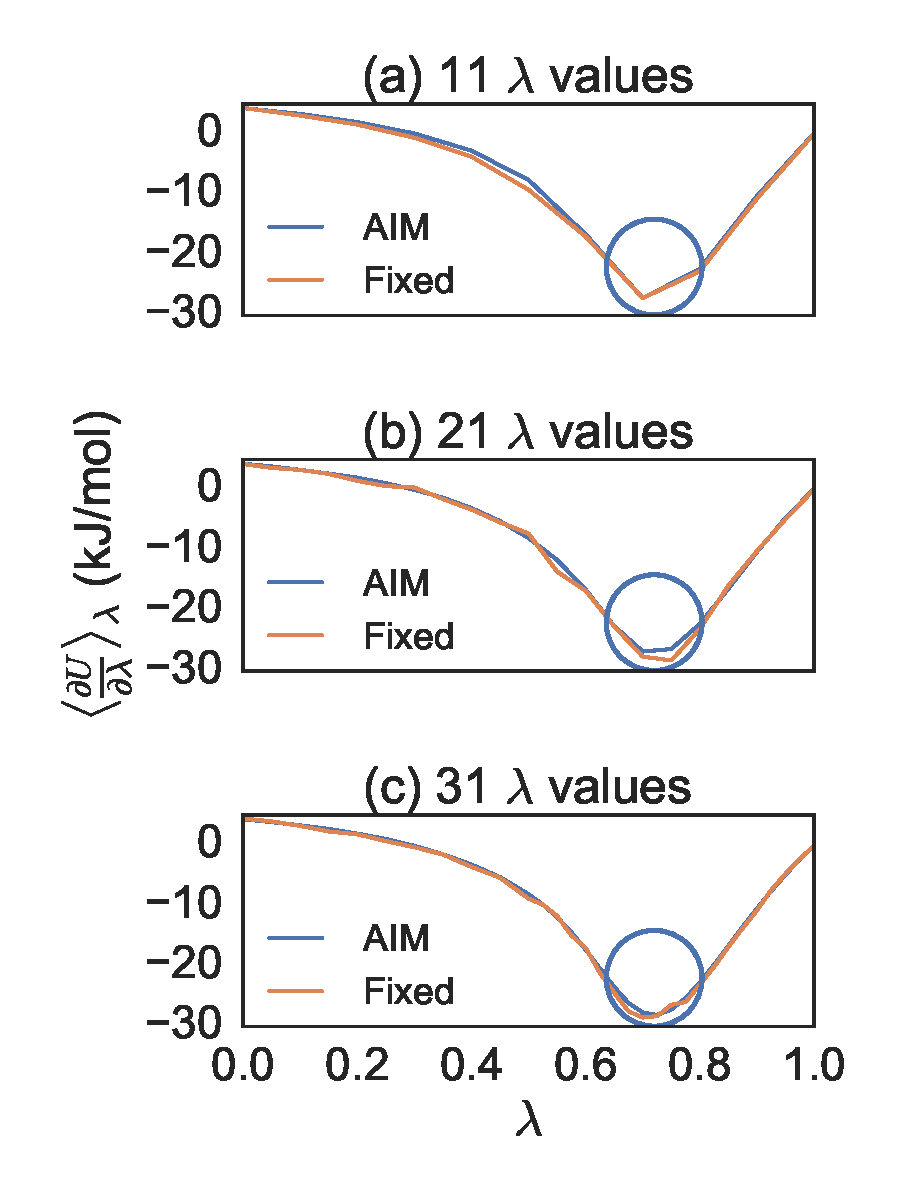
\includegraphics[width=0.5 \textwidth]{All_lambdas_at_100ps_per_lambda}
    \caption{Methane solvation free energy results. Eight trial simulations of 100 ps per $\lambda$ for 11, 21 and 31 $\lambda$ values. This shows how the number of $\lambda$ values were chosen to effectively compare AIM to fixed $\lambda$ simulations. The circles indicate the region where the $\lambda$ density needed to be increased.}
    \label{increasinglambdas}
\end{figure*}
\pagebreak


\begin{figure*}[htbp]
    \centering
    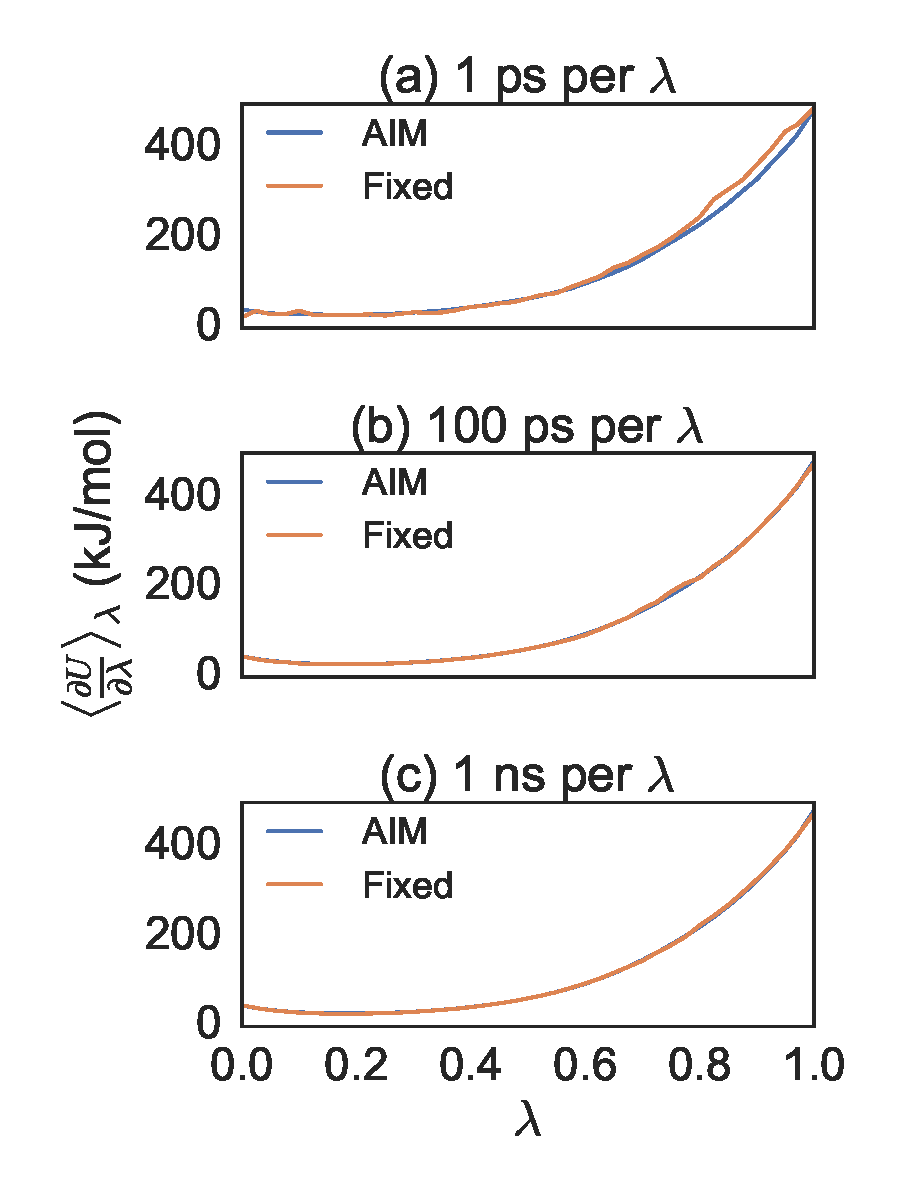
\includegraphics[width=0.5 \textwidth]{tripep_lambdas}
    \caption{Alanine to valine mutation free energy. Eight trial simulations of 41 $\lambda$ values at 1 ps, 100 ps and 1 ns per $\lambda$. Note the smoothness of AIM versus fixed $\lambda$ simulations. AIM requires less samples than fixed $\lambda$ simulations to smooth the free energy function.}
    \label{a2vlineplot}
\end{figure*}

\pagebreak

\begin{sidewaysfigure*}[htbp]
    \centering
    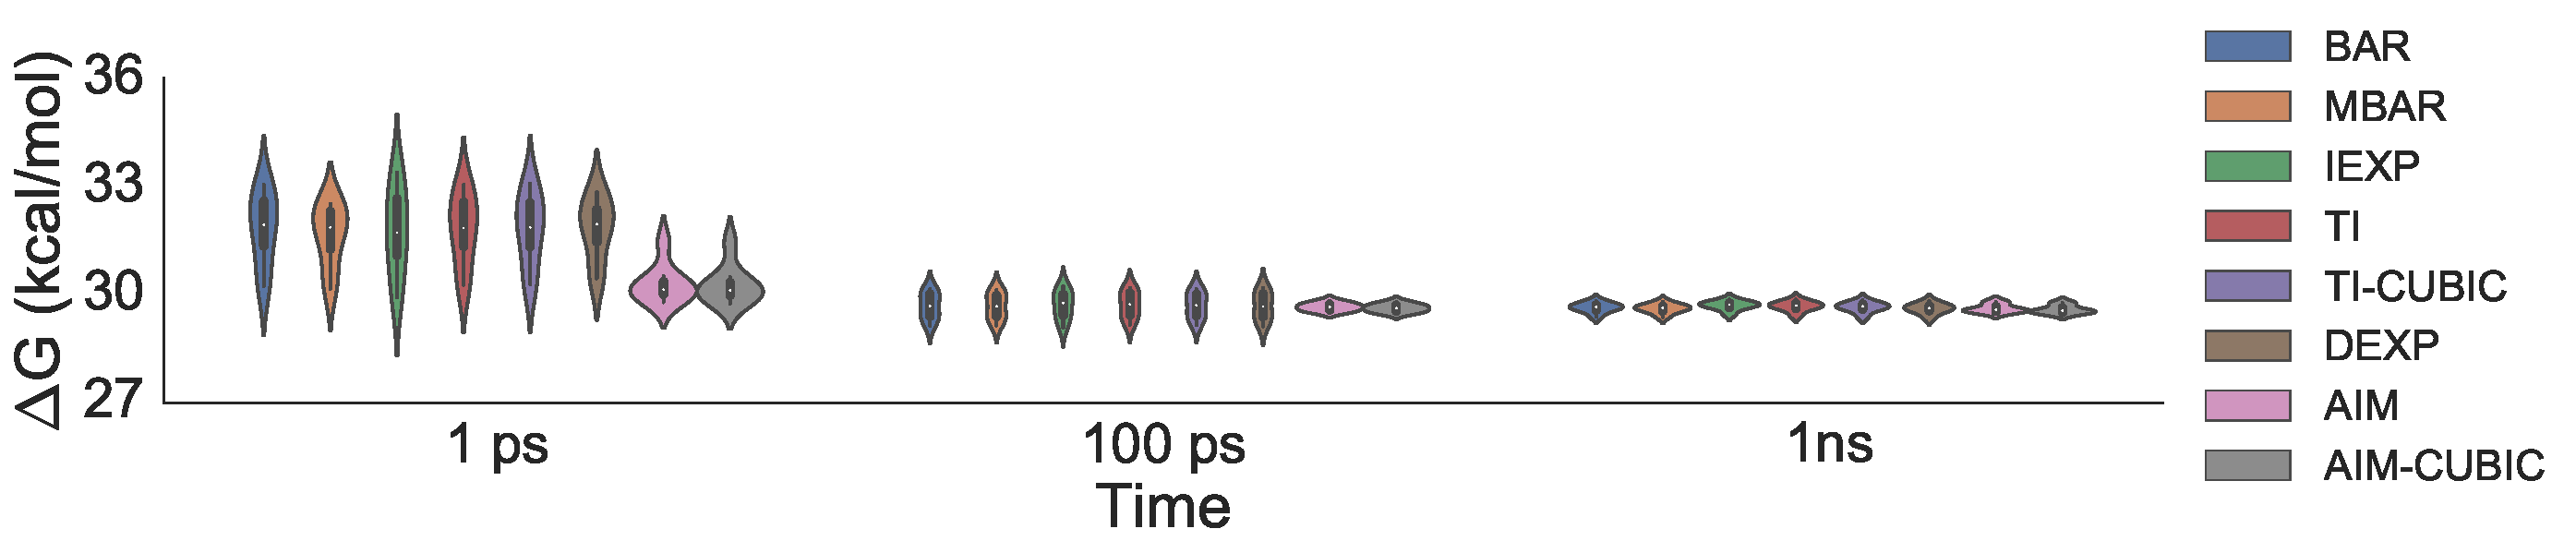
\includegraphics[width=1\textwidth]{A2V_41L_violinplotovertime}
    \caption{Violin plot showing alanine to valine mutation results for 41 $\lambda$ values averaged over eight trials. The graphic shows all methods have similarly converged at 1 ns per $\lambda$. Note that AIM and AIM-CUBIC converge more rapidly than other methods and are mostly converged at 100 ps per $\lambda$}
    \label{a2vviolinplot}
\end{sidewaysfigure*}

%%%%%%%%%%%%%%%%
% Chapter 3
%%%%%%%%%%%%%%%%

\chapter{Design Considerations for Implementing Halbach Arrays and High Temperature Superconductors for Contact-Free Flywheel Energy Storage Systems}
Christopher Mirabzadeh, Chris Birkinbine, Daniel Schneider, Joe Law, and Christine Berven

\begin{center}
Manuscript submitted on Sept. 2017 to \textit{IEEE Transactions on Applied Superconductivity} - Manuscript ID TAS-2017-0187
\end{center}

\section*{Abstract}
We have investigated the use of Halbach magnet arrays in combination with Type II High-Temperature Superconductors for use as a levitating thrust bearing for a fly-wheel energy storage system. Halbach arrays were selected because they have effectively one-sided flux and a greater flux gradient which would be expected to result in a greater levitation force and effective restoring force stiffness; each being beneficial in the design of such a system. To find the optimum orientation of the magnets for the arrays, we used Infolytica Magnet, a finite-element computation software package, to iterate over all permutations of magnet arrays costing of 3 and 5 magnets of single and double layers. The fields and levitation forces as well as the width of the magnet arrays relative to the width of the superconductor were analyzed.  Within our given design constraints, we found that, compared to a single magnet, a single-pole Halbach array was predicted to increase levitation force and stability, reduce stray fields, focus the flux, and increase the bearing stiffness.  We present our findings and suggest guidelines to increase levitation force of a superconducting magnetic bearing with qualifiers and rationale for optimizing such a system.  

\section{Introduction}
The NASA-sponsored, University of Idaho design team was tasked to design and build a solar energy storage system for reliable, efficient, and economical energy storage needs to power a lunar colony. This colony will consume an estimated 525 kW of power. The solar panels chosen as the main method of generating the required electrical energy require exposure to the Sun; however the moon cycles through 336 hours of sunlight and then 336 hours of darkness. During the hours of darkness no power will be generated from the solar panels. The UI design team designed a method to store energy for this period of darkness. 

Batteries, widely used for energy storage applications, were rejected because batteries are very inefficient at low temperatures found on the Moon. Most batteries deliver their power via a chemical reaction that produces electrical energy, when the temperature drops their chemical reaction slows and the battery cannot produce the same current it does at higher temperature leading to possible premature failure of the cell.  In addition, the cycle life, the number of complete charge - discharge cycles a battery can perform, is relatively short. 

As an alternative, chose a flywheel energy storage system for storing the required energy. Flywheels work by storing excess electrical energy as kinetic energy in a rotating system which may be stored for long periods of time or taken out as needed. Flywheels are environmentally clean, contain no hazardous materials, can efficiently store energy for long periods of time, have a long life expectancy (greater than 20 years), are ideally suited to multiple power applications, can handle rapid discharge rates without degradation, and are easier to maintain versus other options. Flywheels are typically constructed of steel and rotate on conventional contact bearings; however, contact bearings incur energy losses from friction.  The UI design team chose to use magnetic levitation via high temperature superconducting (HTS) magnetic bearings because it has been suggested as a method to remove those energy losses \cite{xia, miyazakim, fang, cansiz, strasik, sung, sotelo2, nagashima, birkner, werfel, coombs002, ma, mulcahy1,choi}. 

High temperature superconducting magnetic bearings (SMB) have challenges of their own.  First, it is very difficult to control free bearings as they are analogous to a spinning top with no fixed point and multiple degrees of freedom.  Second, an SMB may have its natural resonant frequencies stabilized with the aid of an active magnetic bearing or by the mechanism of flux trapping.  Additionally a superconducting magnetic bearing will have a decrease in levitation force over time due to flux creep \cite{miyazakim, suzuki, postrekhin}.  There are also rotational energy losses that must be considered because SMB's are not completely friction free.  There are at least three sources of energy loss\cite{xia, sotelo2}; (a) windage due to motion of the rotor in a fluid, (b) thermal losses from radiation, convection and conduction and (c) hysteresis losses due to inhomogeneities in the magnetic field.

\section{Methods}
The UI Design team chose to use superconductor bearings instead of traditional bearings because they are materials that conduct electricity with zero resistance and completely expel magnetic fields when cooled below a characteristic critical temperature. This makes HTS attractive since these temperatures are easily accessible using Liquid Nitrogen. All superconductors expel magnetic fields when cooled below a characteristic critical temperature. The critical temperature of type I superconductors require temperatures well below 77K, whereas the critical temperature of type II high temperature superconductors is well greater than 77K. The difference between a Type I and Type II superconductor, besides the critical temperature, is that Type II superconductors have two critical fields.  Between the critical fields lies a mixed-state where the superconductor traps magnetic flux and hence the Meissner Effect is not complete.  Thus, high temperature superconductors cooled with Liquid Nitrogen can be used to stably levitate permanent magnets. For a review of superconductors and their properties see Tinkham \cite{tinkham}.

 A number of authors have already explored superconducting magnetic bearings and flywheel energy systems \cite{xia, miyazakim, cansiz, sung, nagashima, werfel, coombs002, ma, mulcahy1, turner, ikedia}.  In addition, Halbach arrays have been optimized for use by Maglev levitation vehicles \cite{Jing, deng, zhang, del2, liu, deng2} and in motor designs \cite{turner, soltner, robertson, wang}.  In this section we mean to present our procedure for selecting the appropriate magnetic array for all of our requirements and constraints.  We then present several different array configurations based on these preliminary findings based on Finite Element Analysis (FEA) methods and finally experimental methods to confirm and rationalize the final recommendations.

The levitation force must be large enough to support the rotor mass we must consider practical constraints such as size and spatial volume.  Selecting neodymium permanent magnets were chosen because of their high residual magnetization and because  small volume permanent magnets will always outperform iron core electromagnets in a small dimension space\cite{hawkins}. Selecting these magnets enabled us to increase the relative force per volume ratio which reduces the number of magnets needed for levitation.  For the initial phase of the project we considered using alternating magnetic rings such as those used in similar projects \cite{strasik, sotelo1}.  Calculations proved such a magnet to have sufficient force to levitate our rotor design; however, the design and manufacture was deemed cost prohibitive.  Instead, we researched smaller, “off the shelf”, magnets.  We further discovered that stray flux could be decreased and magnetic stiffness increased if we formed the magnets into radial Halbach arrays.  

A Halbach array, also called a “flux sheet” by Mallinson \cite{mallinson}, is a simple arrangement of permanent magnets that effectively doubles the field on one side, the active face, and reduces stray fields on the opposite side, the “inactive face”.  See Fig. \ref{fig_halbach} for a simple arrangement.  Halbach arrays are common in brushless motors \cite{Hull1, zhu} and are seeing an increased use in magnetic levitation rail trains \cite{ham, Jing, post}, flywheel energy systems \cite{sotelo2, turner}, and Nuclear Magnetic Resonance (NMR) \cite{raich, soltner}. Also, since the field is reduced on the inactive face, we expect use of Halbach arrays to be beneficial in reducing the magnetic interference between the rotor and stator.  

One of our goals was to produce as much magnetic force as possible per unit area.  There is computational and experimental evidence that the Halbach array superconductor system is superior to a permanent magnet and superconductor system \cite{sotelo2, Hull1, Jing, turner, del1, deng, zhang, del2, liu, deng2}.  A levitating halbach system shows increased levitation force, increased stiffness and enhanced stability.  On average the levitation force between a halbach array and superconductor has been shown to be 2.3 times that of a single permanent magnet and superconductor \cite{Jing}.  FEA shows that the Halbach array configuration is capable of obtaining the same magnetic force for larger gaps between rotor and stator as compared to using iron shim flux shapers \cite{sotelo2}.

Maximum levitation force is attainable by first cooling the superconductor far from any magnetic field \cite{ma, Hull1999, del1, zeisberger2}.  This is called zero-field-cooling (ZFC). Flux Creep causes time relaxation in the levitation force.  This problem is resolved by preloading the SMB before initial rotation \cite{miyazakim, suzuki, postrekhin, ma}.

Cooling the superconductor near a magnet source is called field cooling (FC) and although this configuration has been shown to  reduce the levitation force, it improves the lateral stability due to pinning \cite{ma, Hull1999, del1}.
A field cooled system is less susceptible to flux creep because the HTS resists any changes in the external field \cite{xia}.

Werfel et al. have emphasized design rules for HTS bearings \cite{werfel}.  
\begin{quote} 
Acheiving high bearing stiffness requires a multipole arrangement of the magnets.  If the air gap is larger than 4-5 mm, due to magnet bandage or thermal isolation, a reduced number or even a single magnet pole may give better force-density values. 
\end{quote}

It has been recognized that edge effects between superconductors and magnets directly affect the levitation force \cite{ma, Jing}.  Therefore the width ratio, fixed width halbach array versus variable width HTS, and field cooling height must be considered a characteristic of the overall system specifications.

Del-Valle \cite{del1} have shown that as the ratio of the width of the superconductor to the magnet array increases so does the stabilizing force; however, when the width is large enough as to completely cover the total width of the magnet array simpler arrangements may be the better configuration due to the magnetic field profiles.  Furthermore, they suggest having a height of the permanent magnet larger than that of the superconductor.

In an evacuated system we may ignore windage and thermal losses except by radiation; however, magnetic hysteresis loss has been shown to depend on the amplitude of changes in the B-field on the surface of the superconductor \cite{coombs003}.  This implies that any changes in frequency, which creates a change in the B-field at the surface of the superconductor, will create rotational losses.  These hysteresis losses are analogous to frictional drag \cite{ma}\cite{turner}.  Inhomogeneities in the magnetic field of the permanent magnets lead to time-varying magnetic fields on the surface of the superconductor, i.e. a conductor moving through a non-uniform magnetic field induces eddy currents and thus contributes to energy losses.

Spin up and spin down tests have shown rotational losses to be a function of temperature and height between a rotor magnet and superconductor \cite{cansiz,  werfel}.  It was shown that the smaller gap distance, 4mm compared to 5mm, increases hysteresis losses due to higher field variations experienced by the superconductor.  The observed decay rate in the spin down test has been used to approximate a relative coefficient of friction with a range in magnitude from $10^{-5}$ to $10^{-8}$ \cite{cansiz}

\subsection{Computational}
Based on the selection criteria outlined above we considered arrays made of 3 and 5 permanent magnets to produce a target levitation height greater than 5 mm. Three magnets can be used to create a single pole and five to create a double pole.  In order to determine the greatest levitation force per unit area, different magnet orientations were simulated using finite element analysis with the finite element package Infolytica - MagNet, version 7 \footnote{http://www.infolytica.com/}.  Only the levitation force was considered.  ZFC and the Meissner effect are assumed.  Idealized materials restrict our simplified model to closer resemble Type I superconductors.

Orientations considered were all possible permutations of 3 and 5 magnet arrays such as those pictured in Table \ref{tab_nonlin}.  Other configurations included separating the magnets with iron shims, and 1 layer  versus 2 layers as 2 layers will have a height larger than that of the superconductor as suggested by Del-Valle \cite{del1}.

\begin{table}[ht]
\caption{Proposed magnet arrays} % title of Table
\centering % used for centering table
\begin{tabular}{cc} % centered columns
\hline % inserts single horizontal line
\
\\
$90^\circ$ Roll Angle & $\uparrow \rightarrow \downarrow \leftarrow ...$ \\ % inserting body of the table
\\
Alternating Iron(I) Shims & \framebox{I} \framebox{$\rightarrow$} \framebox{I} \framebox{$\uparrow$} ... \\
\\
Iron Shims Outside the array & \framebox{I}  \framebox{$\rightarrow$} \framebox{$\uparrow$} \framebox{$\leftarrow$}  \framebox{I}\\
\\
1 Layer & \framebox{$\rightarrow$} \framebox{$\uparrow$} \framebox{$\leftarrow$}\\ [1ex] % [1ex] adds vertical space
\\
2 Layers &  \framebox{$\rightarrow$} \framebox{$\uparrow$} \framebox{$\leftarrow$} \\
& \framebox{$\rightarrow$} \framebox{$\uparrow$} \framebox{$\leftarrow$} \\
\\
\\
\hline
\end{tabular}
\label{tab_nonlin} % is used to refer this table in the text
\end{table}

Fully 3D periodic boundary conditions were possible but not necessary to find the desired results.  Slab boundary conditions are useful for simulating a part of a system of planar surfaces (e.g. x and y) with periodic boundaries while leaving the third (z) direction remaining vacuum to infinity.  The model is shown in Fig. \ref{fig_2DModel}.  As shown, the model is 2D which assumes an infinite z dimension. Unless otherwise stated, the HTS was 35 mm wide and 6.35 mm tall.  The magnets were 6.35 mm cubes in order to represent easily obtainable "off-the shelf" magnets.  This limited the angle between any adjacent pole to multiples of $90^{\circ} $.

The 2D simulation is limited, however, Type II superconductors can be modeled with a magnetic permeability less than that of air.  Passive magnetic levitation needs a relative permeability of less than 1.  The relative permeability for the material HTS was set to $10^{-5}$.  This simulates the diamagnetic property of superconductors to oppose an externally applied magnetic field.  The boundary conditions must also be set such that there is zero normal magnetic flux for field cooling.  This allows flux penetration when using a non-linear solver based on the critical state model.  For ZFC the boundary condition is zero vector potential which allows flux to be expelled from the superconductor.

Within the simulation we performed three experiments: 1) Force as a function of height where the HTS positioned 56 mm above each array and was lowered by 1 mm increments.  2) Force as a function of HTS width.  3) Force as a function of array stacks.

\subsection{Experimental}

We purchased 23 seeded, melt growth, superconducting, single domain, YBaCuO (YBCO)  HTS levitation disks for our experiments and flywheel construction from Can Superconductors \footnote{http://www.can-superconductors.com/}.  The wedge shape of the YBCO (Fig. \ref{fig_HTS_Samples}) was pre-selected in order to create a ring when all of the superconductors were fitted together in the final flywheel construction. The HTS were cataloged and referenced as SC0XX, where XX was a number from 01 to 23.  There were no visual defects and all HTS arrived with a clear protective coating. The interaction force between the Halbach array and HTS was measured using the force jig shown in Fig. \ref{fig_forcejig}.  The force jig was constructed of brass in order to limit magnetic interactions.  The force jig consisted of an electro-balance (TREE Model:HRB20001) with a 0.1 g resolution and a 20 kg capacity to quantify the forces.  The interchangeable magnet block assembly, either composed of 8 double layered or single layered periodic arrays in the orientation  $\rightarrow \uparrow \leftarrow$, was placed on the modular tray. The radius of curvature for the block assembly was 3.3375" to the center of the magnets same as the final ring assembly.  We used N-52, 6.35 mm cube magnets purchased from K \& J Magnetics.  The arrays were glued together using a metal compression jig, Gorilla glue, and High-Density Polyethylene (HDPE) to ensure the magnets did not glue to the metal jig. The magnetic field at the surface of the magnets and center of the arrays was measured using a Lakeshore 421 Gaussmeter.  The averages are shown in Table \ref{tab_gauss}.

\begin{table}[htbp]
  \centering
  \caption{Average magnetic field measured with a Lakeshore 421 Gaussmeter and attached Hall probe.  The measurements were taken at the center surface of each configuration shown. }
    \begin{tabular}{rrr}
    \hline
                            & 1 Layer                      & 2 Layers\\
    \hline
   1 Cube Magnet	&	0.555T	&	0.626T\\
   3 Magnets $\uparrow\uparrow\uparrow$		 & 0.581T & 0.644T \\
   3 Magnets $\rightarrow\uparrow\leftarrow$ & 0.750T & 0.834T \\
    \hline
    \end{tabular}%
  \label{tab_gauss}%
\end{table}%

The HTS sample was placed in a plastic cup and secured by a pressure rod.  The magnet block was centered on the modular tray below the cup holder of the force jig. For ZFC, the cup with superconductor was cooled "infinitely" far from the force jig.  As Liquid Nitrogen has a tendency to boil as it comes into contact with warmer solids we allowed the boiling to settle after filling the cup and superconductor and an additional minute passed before placing the cup into the force jig.  Liquid nitrogen was replaced as needed.  The apparatus started at a height of 56 mm and was lowered in 1.25 mm (0.05 in.) increments.  At each increment the scale was read and the force recorded. The HTS were then characterized by their individual levitation force and fit to an exponential function as shown in Table \ref{tab_expfitparm}. 

\section{Results}
For the computational results, flux and force profiles were generated for each permutation of single and double layered magnets using the FEA package. Because we were constrained to off-the-shelf cube magnets, all roll angles between any two consecutive magnets must be  $90^{\circ}$, where we defined the roll angle as the angular difference between two consecutive dipoles. We generated 2176 permutations in all. In order to reduce the number of profiles to be considered we constrained our selection with a set of rules:

\begin{enumerate}
\item Stray magnetic fields may interact with and cause energy losses between the stationary stator and rotating rotor in the air gap between the two.  In order to reduce stray fields and maintain one-sided flux we only considered periodic arrays similar to Halbach arrays.  This means that for any three magnets $A, B, C, A \neq B \neq C$.
\item There is symmetry through the permutations i.e. the orientation $\uparrow \uparrow \leftarrow$ only appeared once but had the same force and flux profile as $\downarrow \downarrow \rightarrow$.  This can be seen in Table \ref{tab_greatforce}. Therefore, profiles with degenerate solutions were unnecessary to consider and discarded.
\item Through consideration of project constraints it was determined that 3 magnets in two stacks would be sufficient to supply the needed force. 
\item It was decided that a potential well of magnetic flux would add some stability despite the fact that we are using ZFC.  Therefore, profiles without the required flux geometry were removed. 
\end{enumerate}

\begin{table}[htbp]
  \centering
  \caption{The data shown here is ordered to show orientations with greatest force profile in the range of interest.  The orientation is that of the magnetic field inside the magnet where U= up, R=right, L=left, and D=down.}
    \begin{tabular}{rrr}
    \hline
    Profile                        & Force(N)                       & Orientation \\
    \hline
    3                              & 4.51                       & UUL \\
    62                             & 4.51                       & DDR \\
    17                             & 4.50                       & RUU \\
    48                             & 4.50                       & LDD \\
    11                             & 4.41                       & ULL \\
    54                             & 4.41                       & DRR \\
    21                             & 4.40                       & RRU \\
    44                             & 4.40                       & LLD \\
    19                             & 4.18                     & RUL \\
    46                             & 4.18                       & LDR \\
    12                             & 4.13                       & ULD \\
    53                             & 4.13                       & DRU \\
    1                              & 3.33                       & UUU \\
    64                             & 3.33                       & DDD \\
    43                             & 3.01                       & LLL \\
    22                             & 3.01                       & RRR \\
    \hline
    \end{tabular}%
  \label{tab_greatforce}%
\end{table}%

The configurations that best met the above criteria were profiles 12 and 19, shown in Figures \ref{fig_fluxprofile_12} and \ref{fig_fluxprofile_19} respectively. Profile 12 was rejected due to smaller force profile and lacked the desired flux geometry.  Thus, two stacks of 3 magnets with profile 19, Fig. \ref{fig_fluxprofile_19}, were found to be the minimum fit for all arguments of space, volume, force and stability.  The force curve for profile 19 with one and two stacks of magnet arrays are shown in Fig. \ref{fig_force19_one} and Fig. \ref{fig_force19_two} respectively.

Experiments using profile 19 were conducted using the above described force jig.  The results for one and two stacks of magnet arrays are shown in Fig. \ref{fig_force22_one} and Fig. \ref{fig_force22_two} respectively.

\section{Discussion}
An analytical model for forces between superconductors and Halbach arrays in the ZFC orientation can be achieved using the method of images, a qualitative approximation for determining the force between a superconductor and permanent magnet system \cite{perez, yang, kordyuk, saslow, Hull1999, tsuch2}. However, the image method is unable to account for edge effects and irreversible magnetization due to vertical displacements \cite{Hull1999}.  When flux penetration occurs, Bean's critical state model will be needed in order to work out the resistance to motion in all directions \cite{ma, tsuch2, ruiz, bean2, davis, del1}.  In order to create a model for the interaction between a Halbach array and HTS we also needed to consider the theoretical model for the "flux sheet" which deals with the phenomena of one-sided flux as derived by Mallinson \cite{mallinson}.  We could also consider a more rigorous interpretation of the method of images such as in \cite{perez}. 

Intuitively, we expected decreasing values in the force as the distance between the HTS and Halbach arrays increased but at this point we are not speculating as to why and reserve a deeper analysis for future works.  A semi-log plot is most useful when one suspects an exponential fit of the form:

\begin{equation}
F=F_0 e^{(\frac{-x}{x_0})}.
\end{equation}

Thus the experimental data was fitted to a semi-log plot as shown in Fig. \ref{fig_force22_two}.  The resulting graph is a near straight line which reinforced our suspicions.   The data was fitted and the fitting parameters are shown in Table \ref{tab_expfitparm}.

\begin{table}[!t]
  \centering
  \caption{Fitting parameters for experimental force data between the HTS and 8 double arrays of profile 19 arranged in a semi-circle to represent a piece of the flywheel to be constructed. The data starts at a height of 15 mm which is the maximum range of interest.}
    \begin{tabular}{cccc}
    \hline
    & \textbf{$F_0(N)$} & \textbf{$x_0(mm)$} & \textbf{$R^2$} \\
    \hline
    \textbf{SC001}& 18.44& 4.78& 0.9999 \\
    \textbf{SC002}& 19.51& 4.69 & 0.9998 \\
    \textbf{SC003}& 20.58& 4.67 & 0.9997 \\
    \textbf{SC004}& 21.01& 4.59 & 0.9999 \\
    \textbf{SC005}& 20.04& 4.67 & 0.9997 \\
    \textbf{SC006}& 18.67& 4.90 & 0.9995 \\
    \textbf{SC007}& 18.45& 4.86 & 0.9997 \\
    \textbf{SC008}& 18.75& 4.73 & 0.9999 \\
    \textbf{SC009}& 20.1 & 4.80 & 0.9997 \\
    \textbf{SC010}& 19.55& 4.78 & 0.9994 \\
    \textbf{SCO11}& 20.65& 4.75 & 0.9996 \\
    \textbf{SC012}& 19.61& 4.82 & 0.9997 \\
    \textbf{SC013}& 19.53& 4.82 & 0.9997 \\
    \textbf{SC014}& 19.82& 4.61 & 0.9997 \\
    \textbf{SC015}& 20.69& 4.65 & 0.9997 \\
    \textbf{SC016}& 19.01& 4.60 & 0.9999 \\
    \textbf{SC017}& 20.53& 4.59 & 0.9998 \\
    \textbf{SC018}& 19.87& 4.55 & 0.9999 \\
    \textbf{SC019}& 18.55& 4.74 & 0.9997 \\
    \textbf{SC020}& 18.39& 4.78 & 0.9996 \\
    \textbf{SC021}& 20.54& 4.63 & 0.9998 \\
    \textbf{SC022}& 18.06& 4.78 & 0.9999 \\
    \textbf{SC023}& 20.41& 4.73 & 0.9996 \\
    \textbf{ Mean}&	19.60&4.72	&0.9997\\
	\textbf{Std. Dev.}	&0.88	&0.10	&0.0001\\
    \hline
    \end{tabular}%
  \label{tab_expfitparm}%
\end{table}%

All of the simulations were solved using the available Infolytica Magnet Static 2D solver. As a 2D approximation neglects fringing and leakage in the material, fringing and leakage in the material and rotational geometry are better simulated in 3D; however, our FEA simulation was strictly used as a means for initial decision making, therefore 2D approximations were deemed appropriate.   Accuracy was further improved by steadily increasing the polynomial order and decreasing the element size of the mesh by automated adaption. 

The simplified 2D model we used was idealistic and closer to the characteristics of Type I Superconductors.  The limitations of the model were: idealized materials, assumed Meissner state, ZFC, only the levitation force was considered, only static solutions, which implies no induced currents from moving magnetic fields therefore AC losses from pinning effects and eddy currents were also ignored. A nonlinear solver was beyond the scope of our initial considerations and not necessary with the assumption of ZFC.  A nonlinear solver was deemed appropriate for the inclusion of pinning and flux penetration in our future works.

Other, stronger configurations are possible, however, not within our given constraints. As shown in Table \ref{table_stacks}, the simulation data predicted that adding additional stacks of the same orientation have the effect of increasing the force but any improvement falls off quickly as the number of stacks increases and is not as great after the third stack. Data using alternating iron shims was excluded due to the lack of required minimum force.  Although iron shims are useful for shaping flux lines the absorption of the field lines into the iron reduces the number of field lines seen by the superconductor, therefore reducing the total force on the superconductor.  Halbach arrays also offer the required flux shapes that we needed.  Different geometries should be considered dependent upon different configuration.

\begin{table}[!t]
\caption{Simulation data of the force between HTS and different layered stacks of array 19 at a height of 6.35mm using FEA}
\label{table_stacks}
\centering
\begin{tabular}{cc}
\hline
Number of layers & Force(N) \\
\hline
One & 4.18\\
Two & 7.93\\
Three & 10.19\\
Four & 11.59\\
Five & 12.49\\
Six & 13.10\\
\hline
\end{tabular}
\end{table}

In comparing the force from array 1 ($\uparrow \uparrow \uparrow $), where all of the magnets are in the same direction, to the force of a dipole magnet of similar volume consider Table \ref{tab_greatforce}.  From the table we may compare profile 1, Fig \ref{fig_fluxprofile_1},  with the configuration $\uparrow \uparrow \uparrow$ to any of the periodic arrays and see that the single direction magnet arrays have less force than any given periodic array.  The force from profile 1 is 1.3 times less than our chosen profile, 19.  

SMB's are typically associated with low bearing stiffness since they can not sustain a large fluctuation in load. Bearing stiffness is defined by how the airgap between the rotor and stator varies under load.  The force between the two opposing surfaces is greatly dependent on the flux density gradient of the airgap. Thus the stiffness of a magnetic bearing would vary as the magnetic field varies. The periodic array focuses the flux to one side of the array creating a more sinusoidal waveform and shortened flux lines due to the interaction between the poles of the individual permanent magnets.  This leads to an increase in the flux density gradient in the airgap.  Further, when compressed, the increased magnetic flux of periodic arrays tend to smooth out the variance in the magnetic field. By increasing flux density and decreasing field variance the periodic arrays have the effect of increasing bearing stiffness. Figures \ref{fig_BFieldSnLs} and \ref{fig_BFiledDbLs} show the higher magnetic field strength of array 19 compared to a single cube magnet and array 1 which represents a rectangular magnet of the same physical volume of array 19.

The original reasoning for increasing the number of layers of magnets was suggested by Del-Valle \cite{del1} in order to have the height of the permanent magnet greater than that of the superconductor and was expected to increase the magnetic field strength.  Our simulations also predicted that increasing the number of array layers would significantly increase the force on the superconductor but our experiments did not mirror the same result.  What we found in comparing the data, Fig. \ref{fig_1layervs2}, is that there was a greater force using multiple layers of magnet arrays at distances greater than 15 to 20 mm.  However, at that point the increase in force fell off to 1.5 times greater and down to near equal force at the heights we are interested in, 5 to 7 mm.  An increase in magnetic field increased the number of flux lines seen by the superconductor.  More flux lines equals more force per unit area, or more magnetic pressure; however, as a ZFC type II superconductor got closer to a magnetic field, flux lines were penetrating and experiencing creep from atomic defects.  Thus intrinsic disorder was of crucial importance in understanding superconducting states.  The decreased force and the slow response to an applied force, which we've seen in the experiments, was likely due to the intrinsic properties of Type II Superconductors. Therefore we saw that more stacks were not advantageous at heights of 5-7 mm. The experiments showed that one stack had a similar force profile as two stacks at short distances.

Given the apparent exponential form for the force as a function of height, we predicted that the effective differential static spring rate would be equal to the negative of the force at a given height divided by the decay length in the argument of the exponent. As could be expected, with a single layer of magnets where the magnetic flux density gradient is larger, the decay length would be shorter which would result in a larger effective spring rate. This can be seen to be consistent with the experimental data, Fig \ref{fig_1layervs2}, in the slopes of the $F(x$) curves at about x = 6mm where the levitation force for both the single and double layer configurations have the same value but the slope is steeper for the single layer case.

When considering stability, our model (and Del-Valle's) showed that the superconductor should be wide enough to completely cover the width of the magnets, Fig \ref{fig_ForceWidthArr19}.  Although the levitation force decreased when the width ratio was above 1 to 1, for the chosen configuration we saw no significant decrease once the width ratio is 1.3 times wider than the magnet array.  Although there was a small decrease in the levitation force, we expected that an increased width ratio maximized the surface area of the magnetic flux seen by the superconductor and therefore maximized the compression area and increased the horizontal stability.  

\section{Conclusion}

The results of a two-dimensional finite element analysis using idealized material properties was assessed and compared to the measured repulsive force between arrays of magnets and high temperature superconductors. The use of Halbach arrays with nearly one-sided flux profiles were investigated with the expectation that this type of flux profile would increase the repulsive force between the magnets and superconductor and increase the effective static spring-rate of the interaction. 

Evaluating the effect of adding additional layers of magnets was also investigated, both experimentally and through simulations. It was expected that the greater flux density would result in both a greater force for all heights and also a greater effective static spring rate. Although the addition of a second layer of magnets did increase the force for most of the height range of interest, an additional layer of magnets did not result in a larger levitation force for the smaller heights and also decreased the differential static spring rate over the whole range of interest. The difference between the measured and simulated forces was possibly due to complications associated with the physics of flux penetration into the superconductor that the model used here was not intended to simulate; however, for initial characterization, the simplified model was found to be sufficient to aid in evaluating permanent magnet array configurations with much smaller investment in software.

A 2D Finite Element Analysis is limited in its ability to predict the interactions between magnets and High Temperature Superconductors.  The simulation data is only appropriate for initial guess work and tells us very little of the underlying physics.  In order to more accurately account for flux penetration and leakage, a 3-dimensional, non-linear solver is required.  On average the levitation force between a Halbach array and superconductor has been shown to be as much as 2.3 times that of a permanent magnet and superconductor\cite{Jing}.  This is due to the one-sided flux created by the rotation angle of the magnetic dipoles.  One-sided flux increases flux density which increases bearing stiffness.  Periodic magnet configurations with increased field gradients are expected to provide higher bearing stiffness.  Therefore, the Halbach array focuses flux, allows for flux control, and increases levitation stiffness.  Simple arrays of 3 magnets are better for maximizing force considerations since in a 3 magnet array there is effectively only one pole, therefore the flux interacts with other poles further away.  To increase the force even more, one may stack the arrays; however, additional layers may decrease the overall bearing stiffness due to flux penetration in type II superconductors and further shortening of flux lines due to pole interactions.  Also, more than two stacks show less of an increase in overall levitation force and considerations should be made for the usable volume space. When considering more stable configurations, width ratios greater than 1.3:1 for superconductor to magnet array shows no considerable reduction in levitation force. The decrease in levitation force due to time dilation caused by flux creep is expected to be minimized by either pre-loading the flywheel before initial rotation or by field cooling.  Pre-loading and field-cooling allows the HTS to better resist any changes in the external magnetic field.


% use section* for acknowledgement
\section*{Acknowledgment}
We would like to thank Infolytica Corporation for the use of their Finite Element Package, MagNet, and Dr. Gilles Fillion for his instructive and timely correspondence.  Funding for this research was provided by The NASA Ralph Steckler Space Grant.

\pagebreak 

\begin{figure}[htbp]
\centering
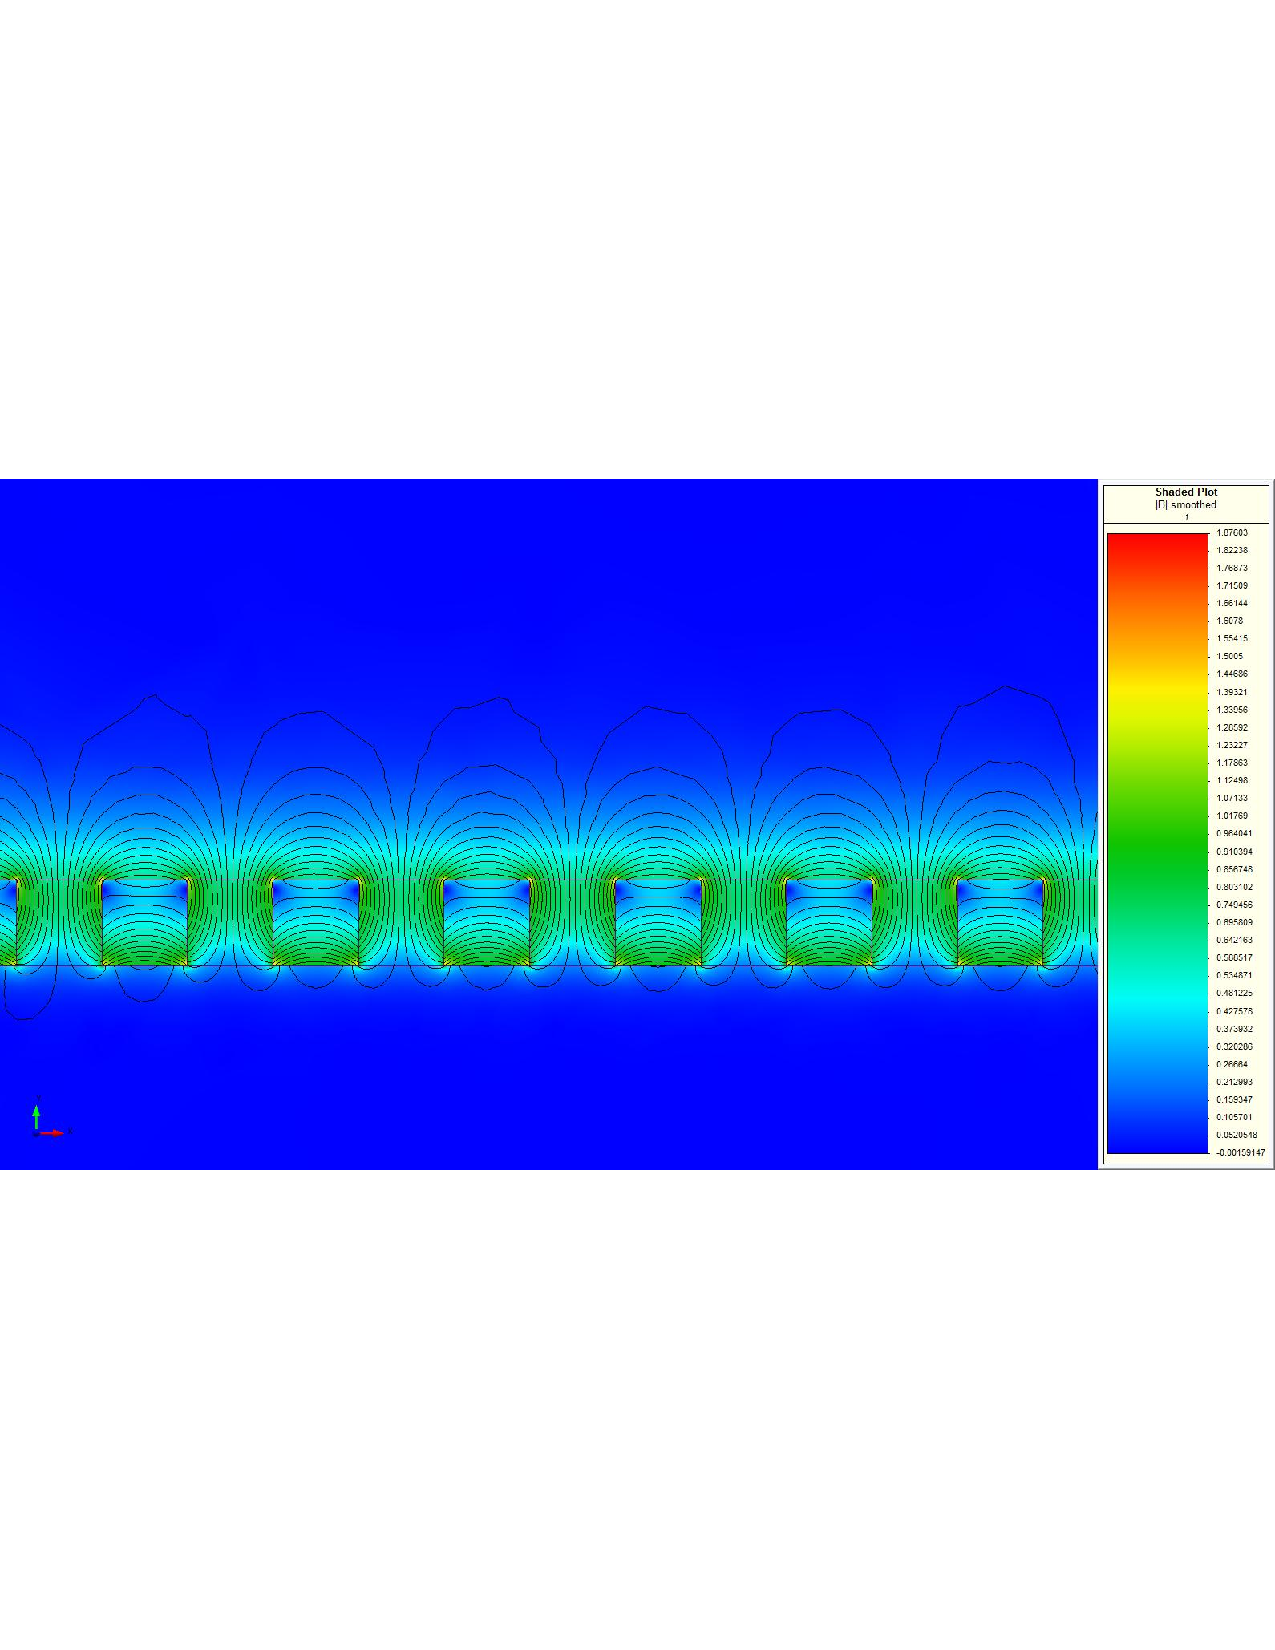
\includegraphics[scale=0.65, clip=true, trim=5cm 10cm 5cm 10cm]{typical_halbach_array.pdf}
\caption{A simulation of an infinitely repeating Halbach array.  The black lines are the flux lines and the gradient colors represent the magnetic field gradient.}
\label{fig_halbach}
\end{figure}

\begin{figure}[htbp]
\centering
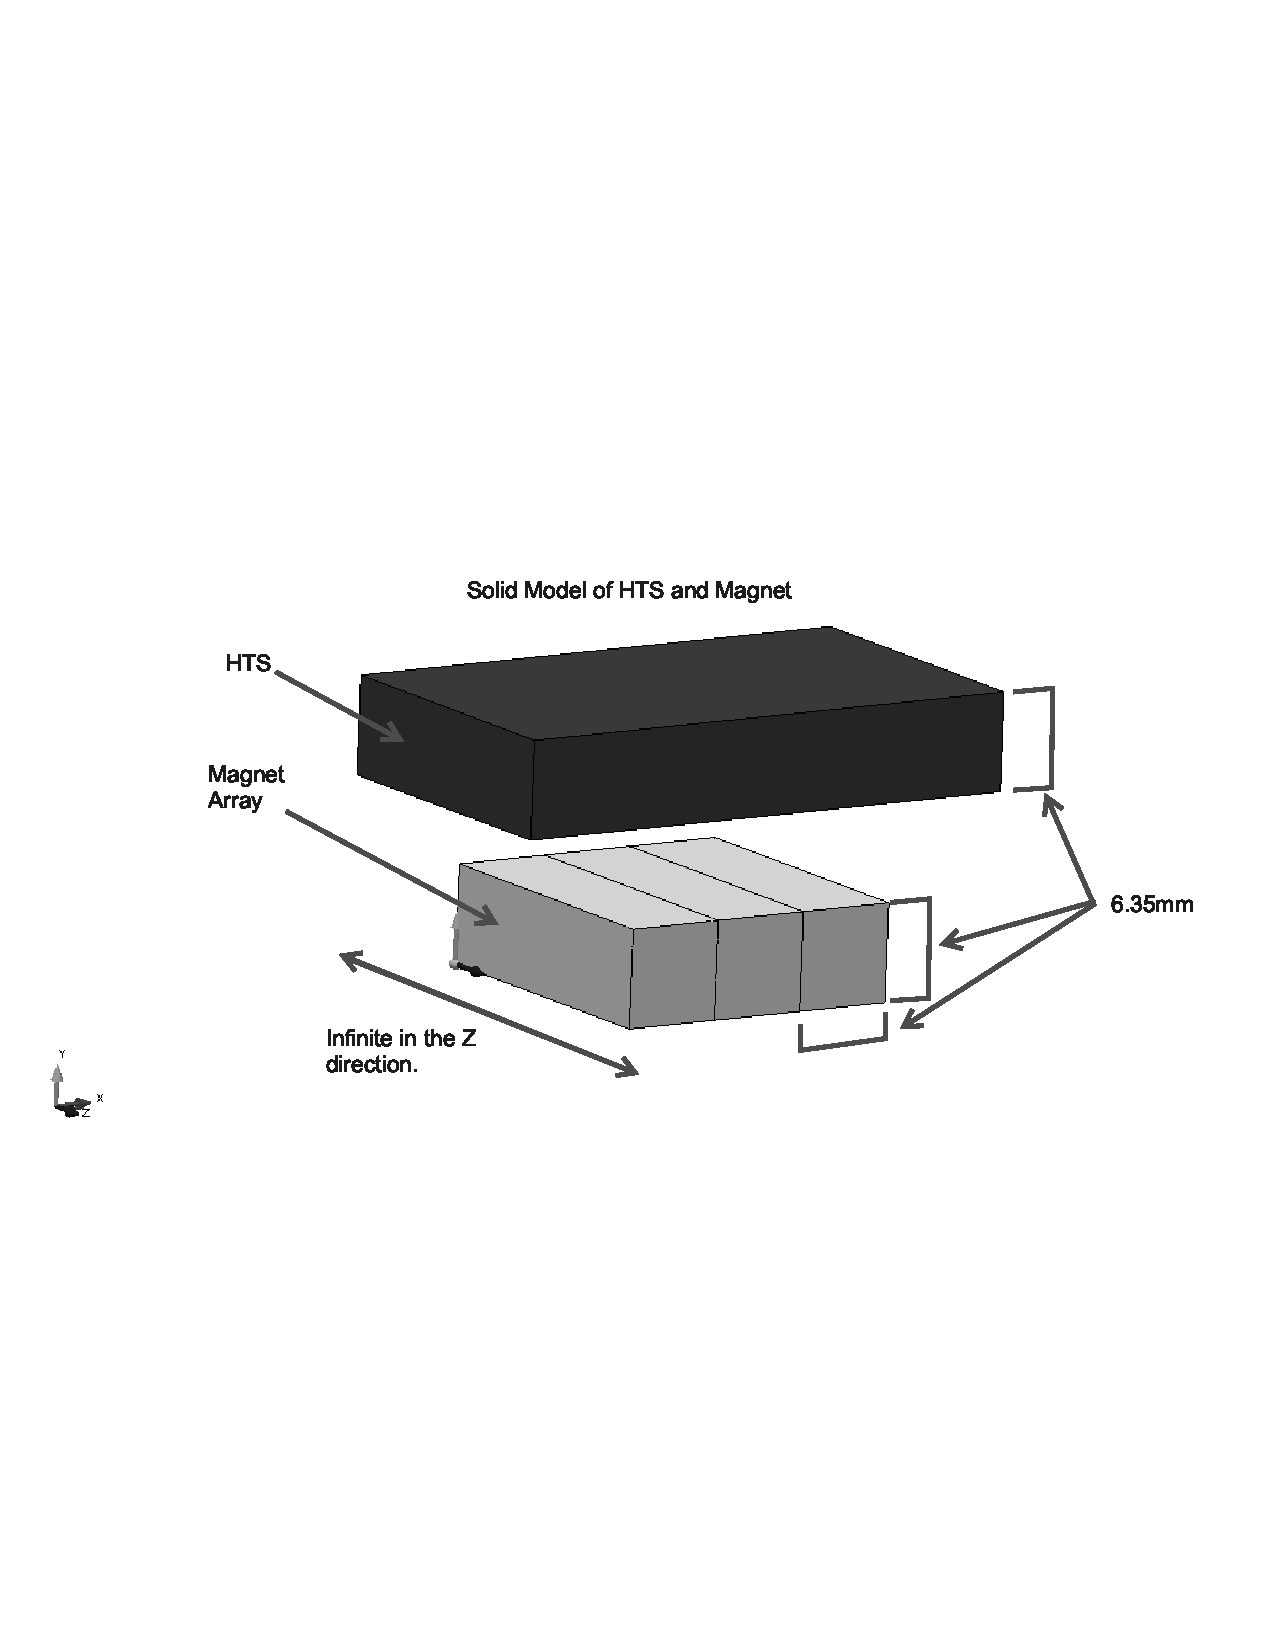
\includegraphics[scale=0.45, clip=true, trim=3cm 8cm 0cm 8cm]{2DModelHTSArray.pdf}
\caption{Two dimensional solid model generated by Infolytica Magnet 7 representing slab boundary conditions with an air box 10 times larger than the unit cell shown.  The z direction is considered infinite.}
\label{fig_2DModel}
\end{figure}

\begin{figure}[htbp]
\centering
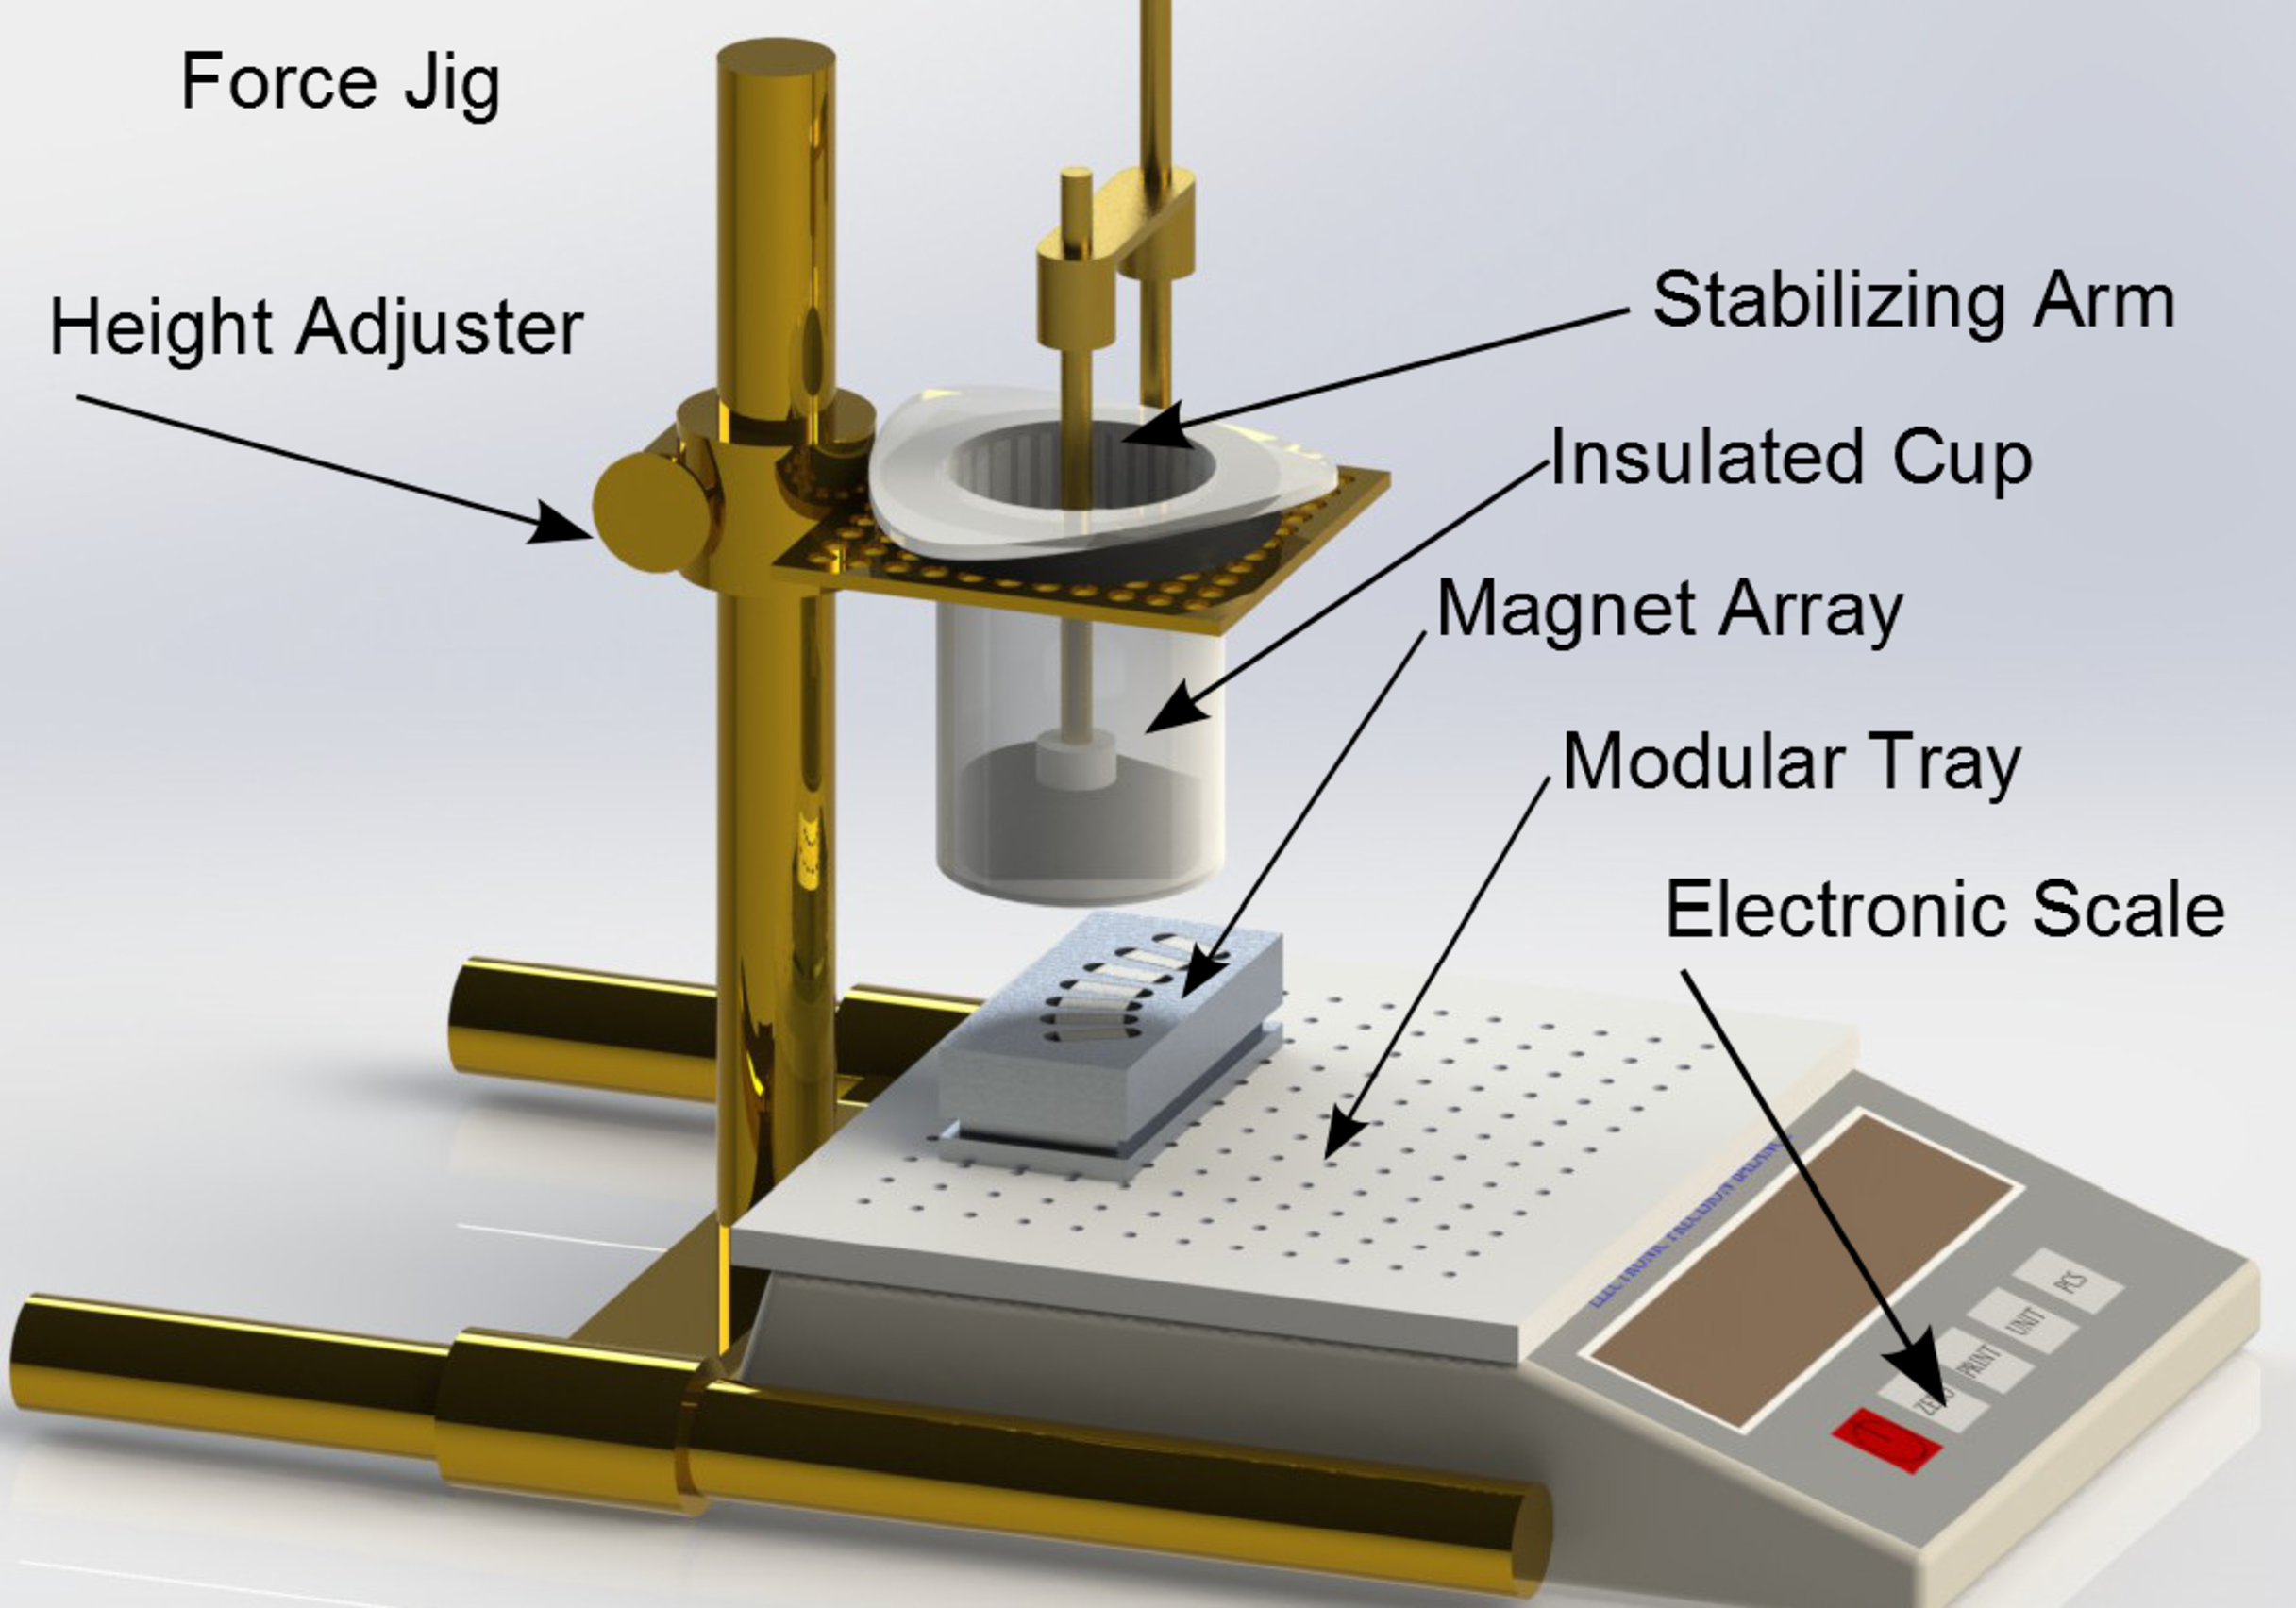
\includegraphics[scale=0.2]{forcejig.pdf}
\caption{Solid model of the Force Jig used to measure the interaction force between superconductors and magnet arrays.  The jig was constructed of brass to maintain low magnetic interference.  The tray of the balance was replaced with a Polythylene modular tray constructed to secure magnet arrays in different orientations as needed.}
\label{fig_forcejig}
\end{figure}

\begin{figure}[htbp]
\centering
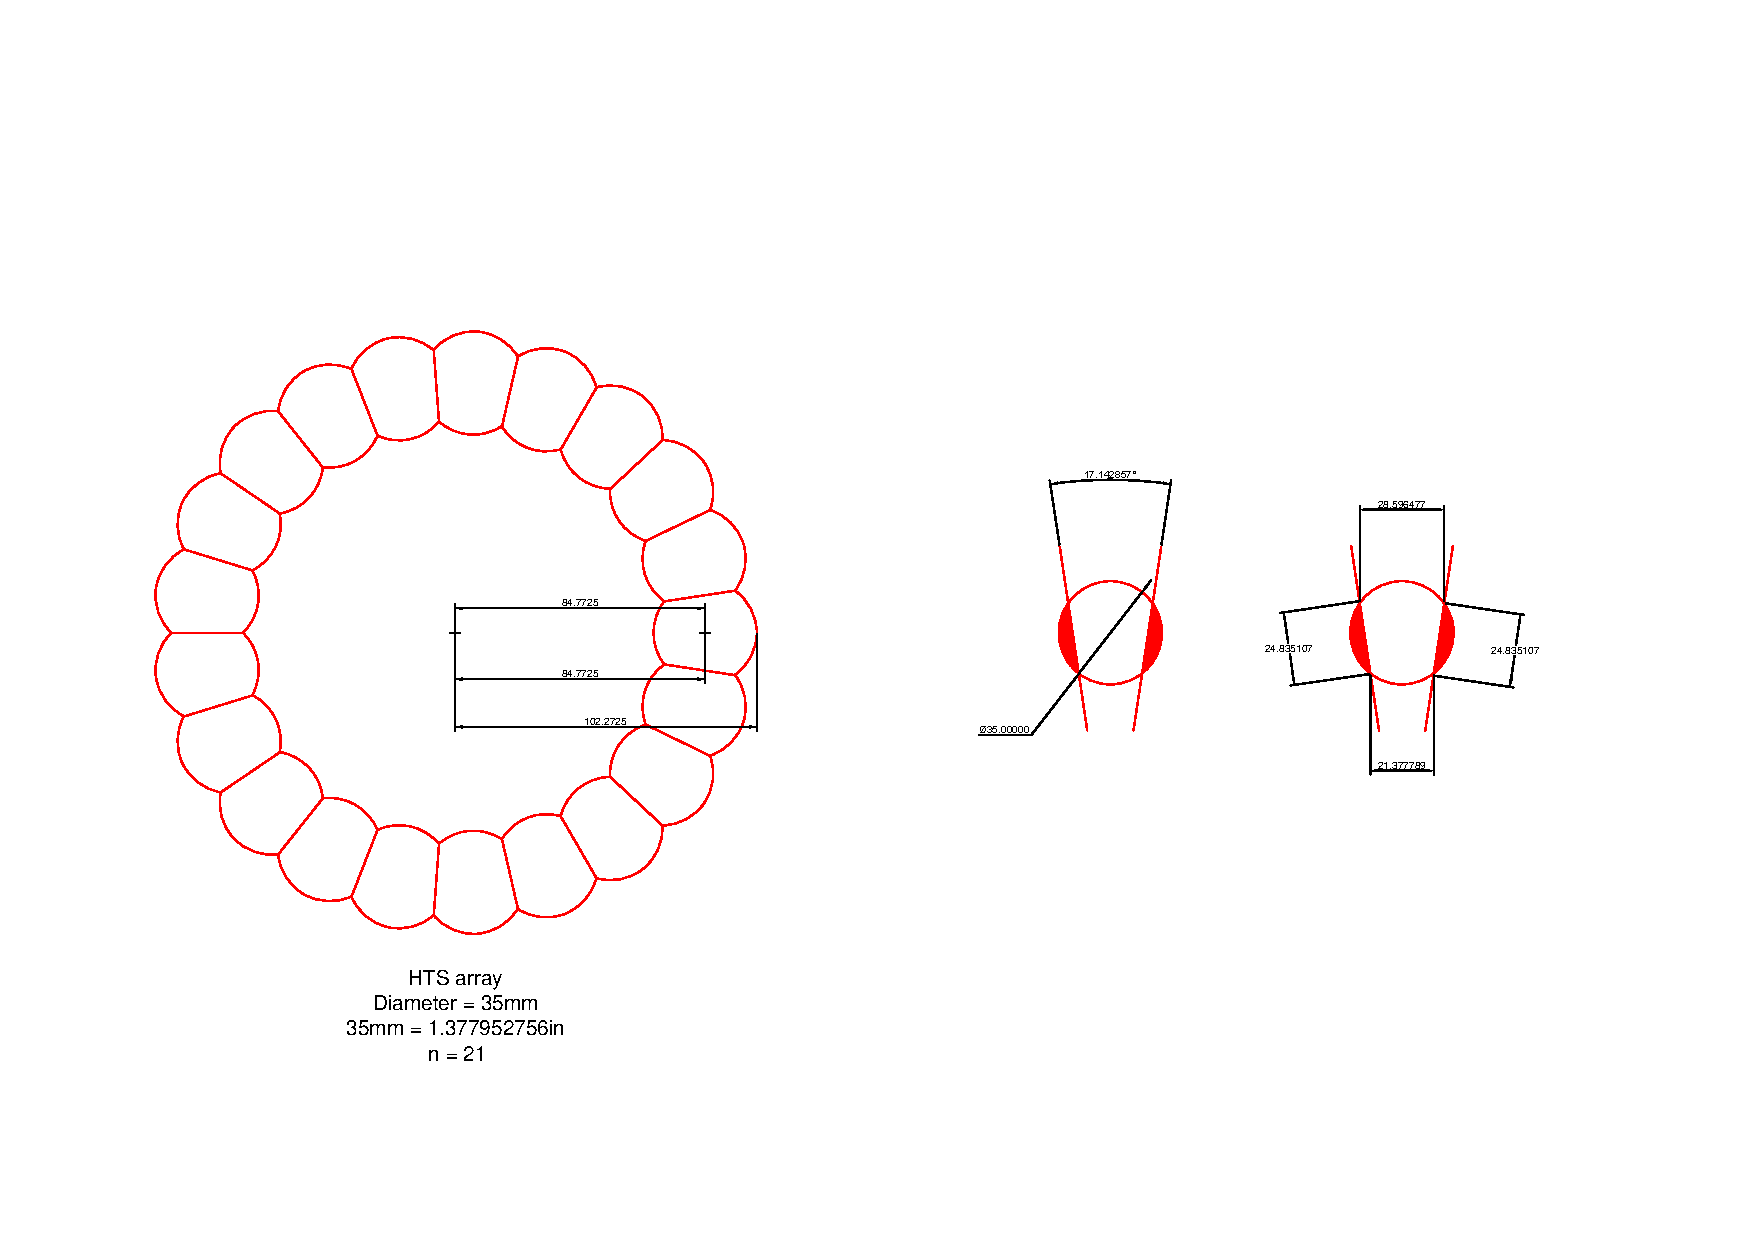
\includegraphics[scale=0.65, clip=true, trim=2cm 3.75cm 15cm 5cm]{HTS_Array.pdf}
\caption{HTS wedge shaped samples cut from Diameter=35mm cylinders ordered from and shaped by Can-superconductors.}
\label{fig_HTS_Samples}
\end{figure}

\begin{figure}[htbp]
\centering
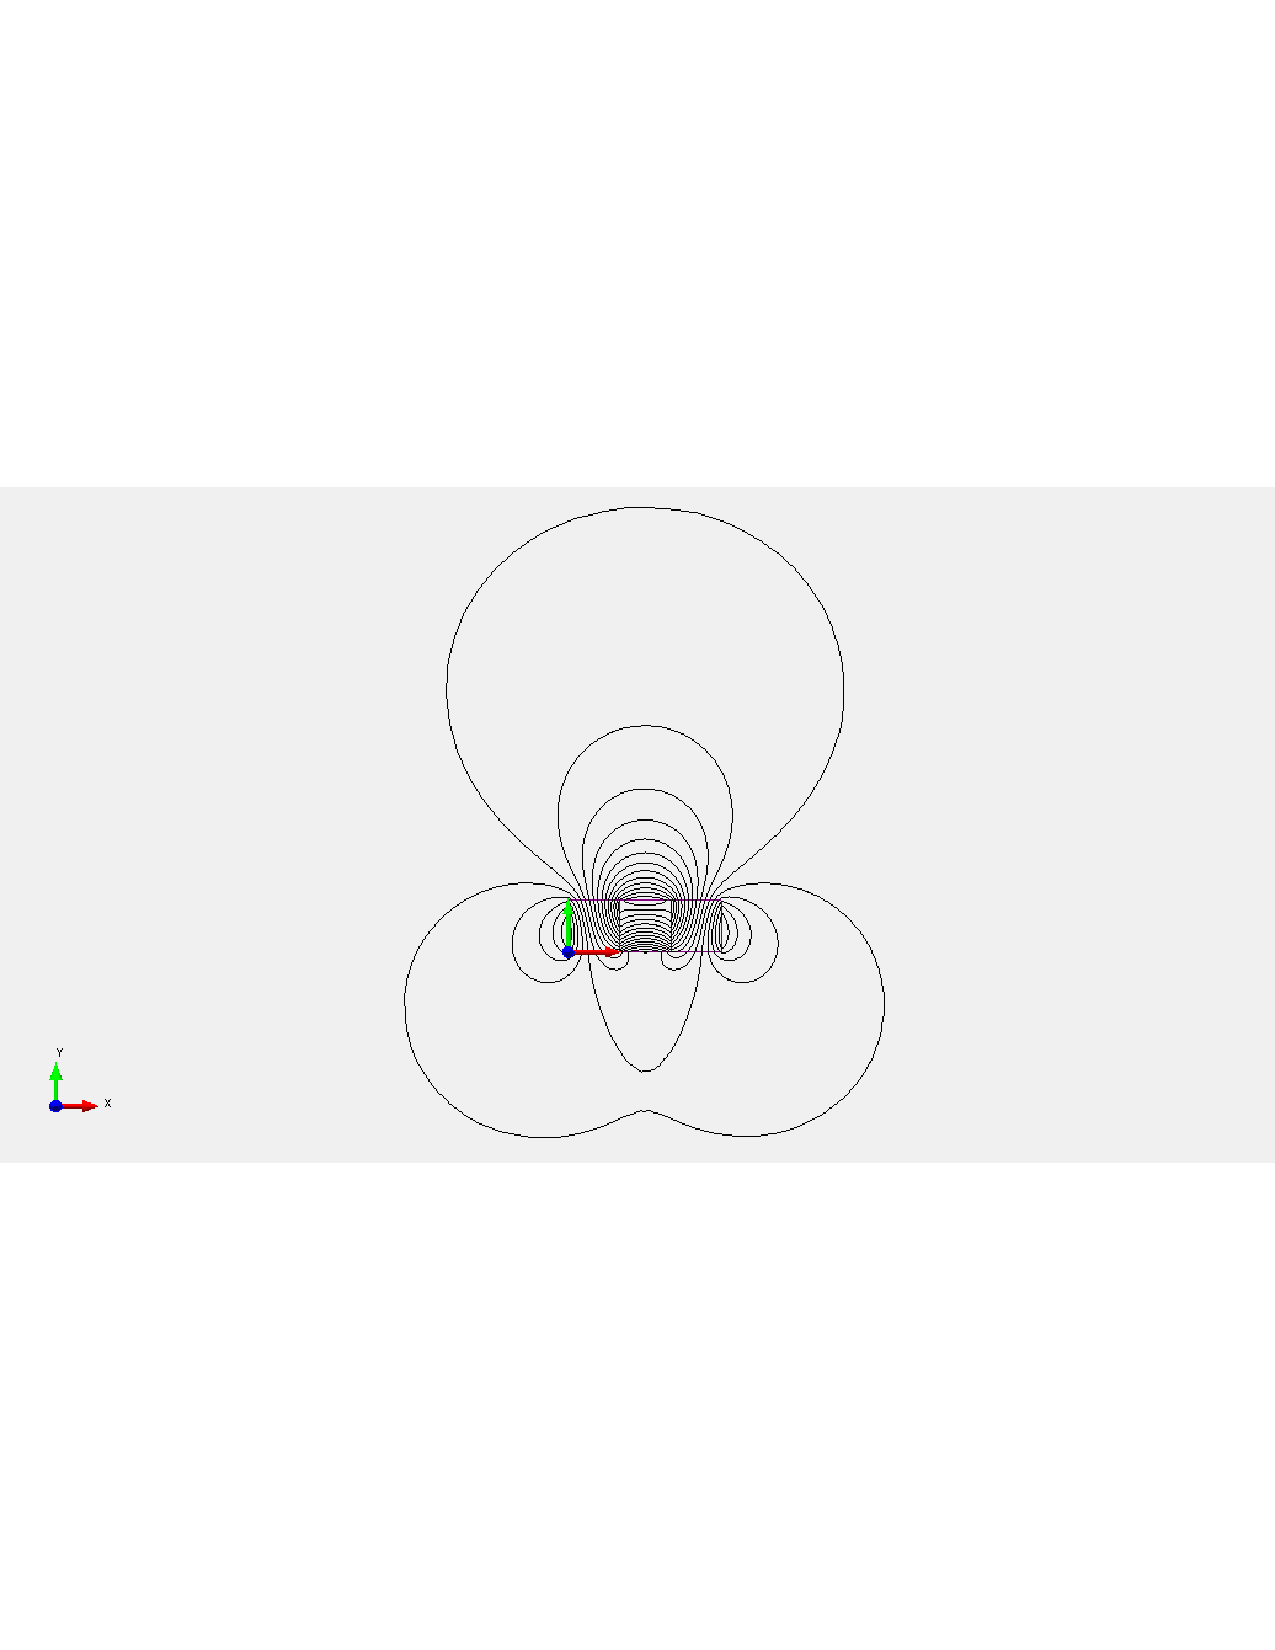
\includegraphics[scale=0.3, clip=true, trim=0cm 5cm 0cm 5cm]{3MagsFluxProfile_12.pdf}
\caption{Flux profile of profile 12 in the orientation $\uparrow \leftarrow \downarrow$.}
\label{fig_fluxprofile_12}
\end{figure}

\begin{figure}[htbp]
\centering
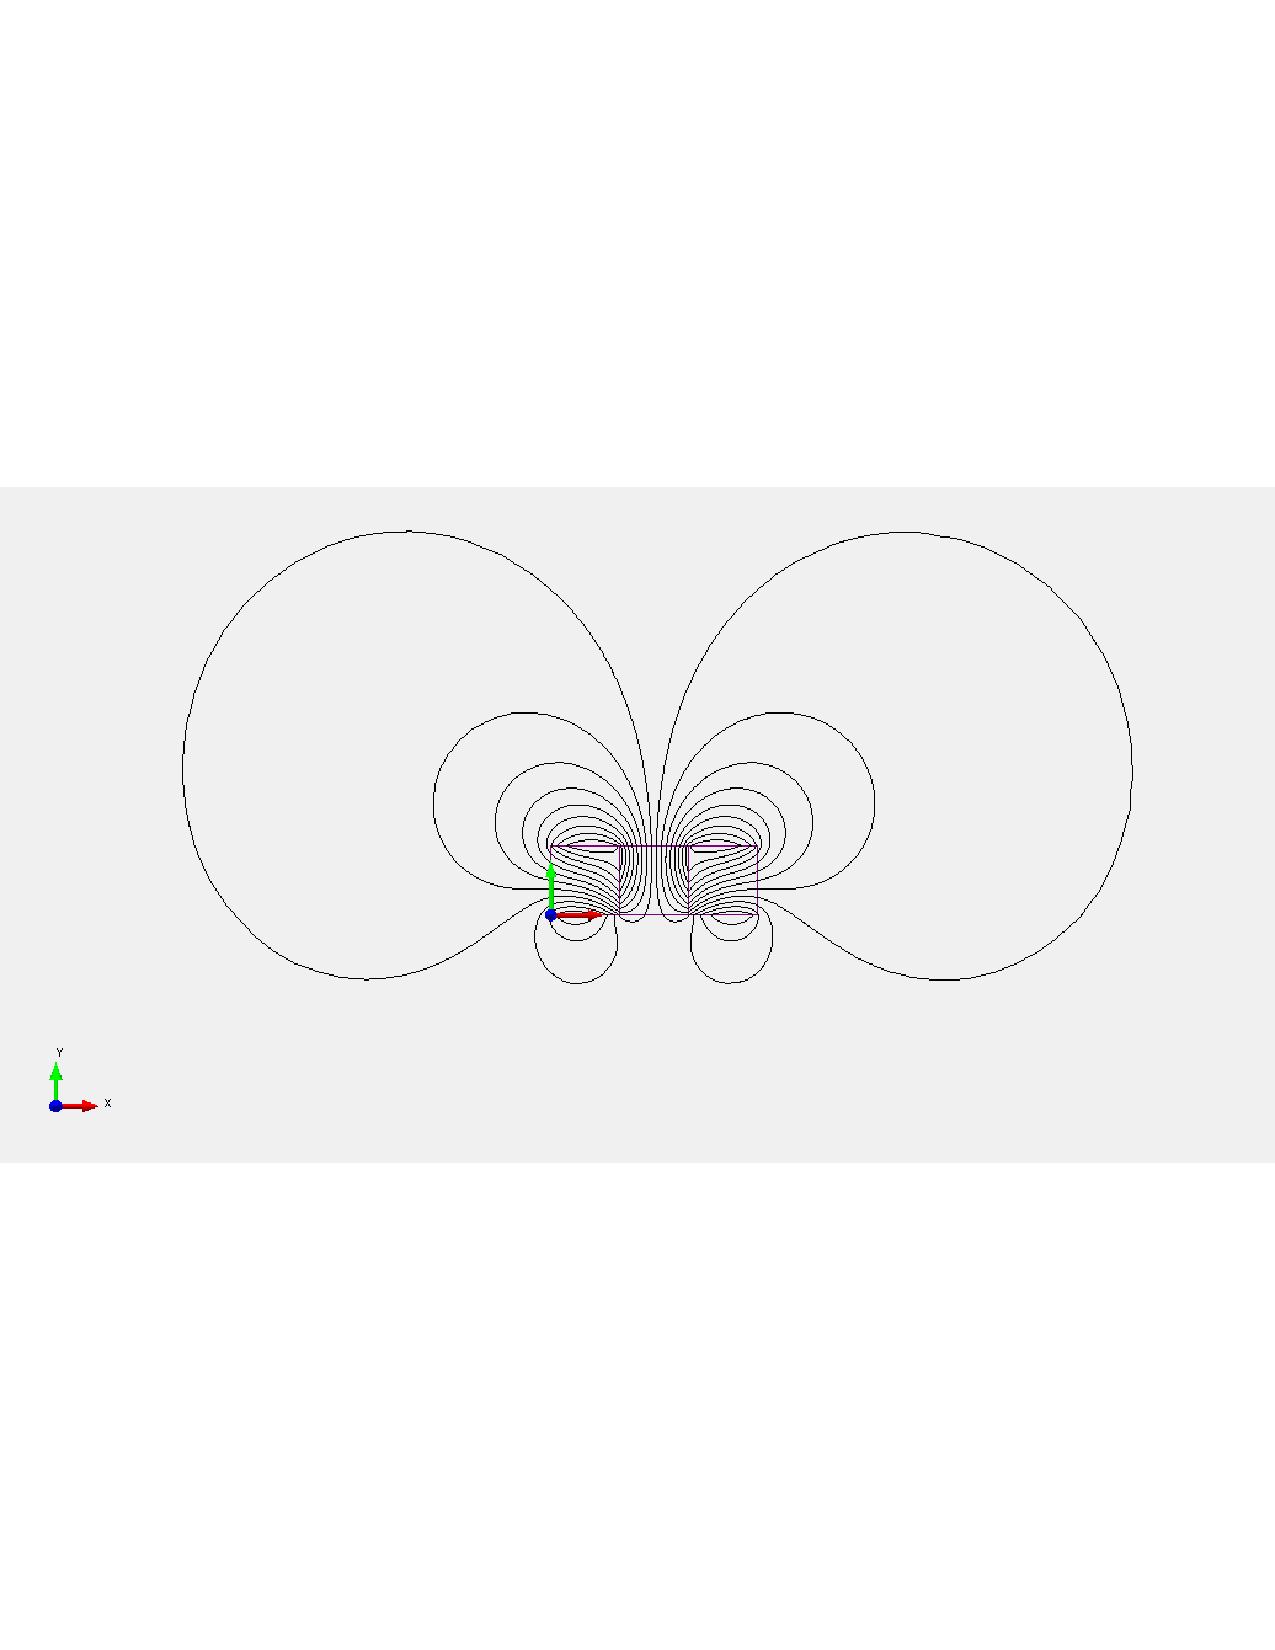
\includegraphics[scale=0.3, clip=true, trim=0cm 5cm 0cm 5cm]{3MagsFluxProfile_19.pdf}
\caption{Flux profile of array 19 in the orientation $\rightarrow \uparrow \leftarrow$.}
\label{fig_fluxprofile_19}
\end{figure}

\begin{figure}[htbp]
\centering
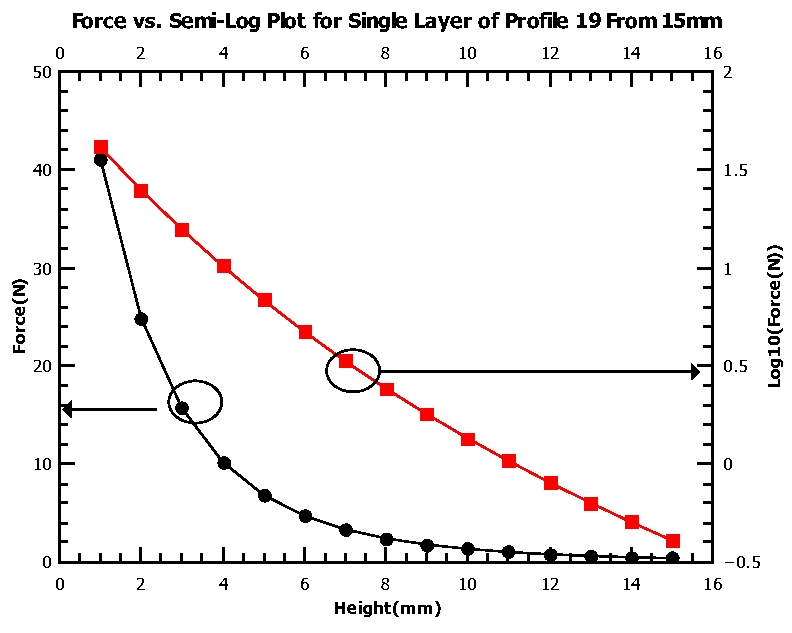
\includegraphics[width=3in]{ForceSemiPro19.pdf}
\caption{Semi-Log plot for FEA using profile 19 in a single layer.  The data was truncated at a maximum of 15 mm for the range of interest.}
\label{fig_force19_one}
\end{figure}

\begin{figure}[htbp]
\centering
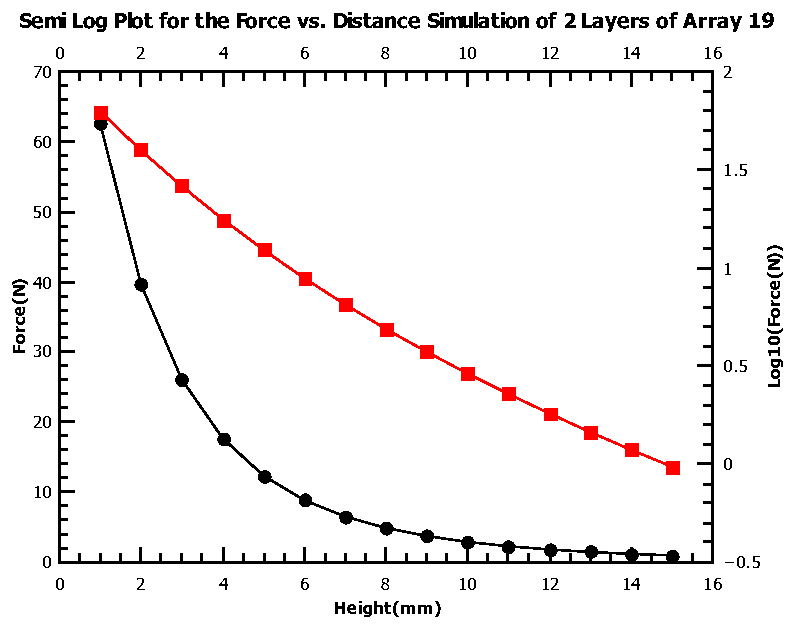
\includegraphics[width=3in]{SemiLogArr192LayersAt15mm.pdf}
\caption{Semi Log plot of the simulation force against two layers of profile 19 truncated at a maximum height of 15mm.}
\label{fig_force19_two}
\end{figure}

\begin{figure}[htbp]
\centering
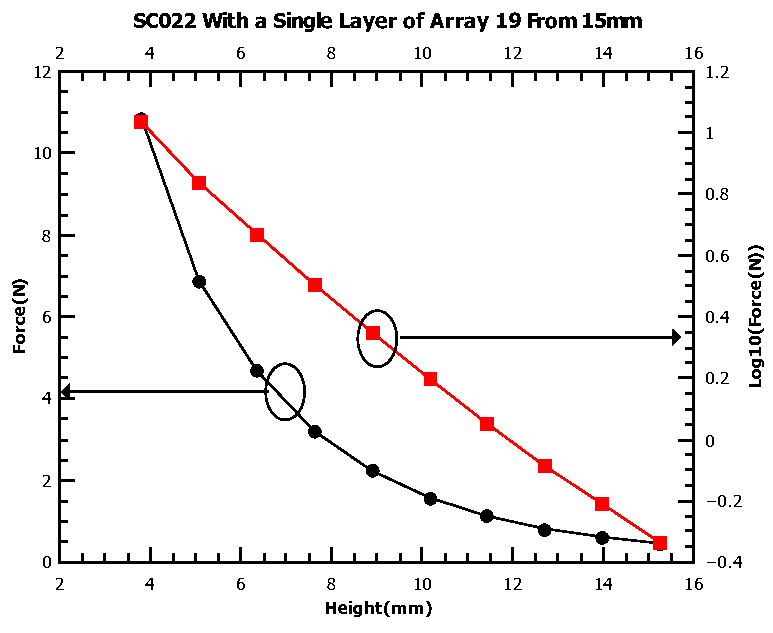
\includegraphics[width=3in]{SC022singleWith19.pdf}
\caption{Semi-Log plot of experiment using SC022 against a single layer of magnets using profile 19.  The data was truncated at a maximum of 15 mm for the range of interest.}
\label{fig_force22_one}
\end{figure}

\begin{figure}[htbp]
\centering
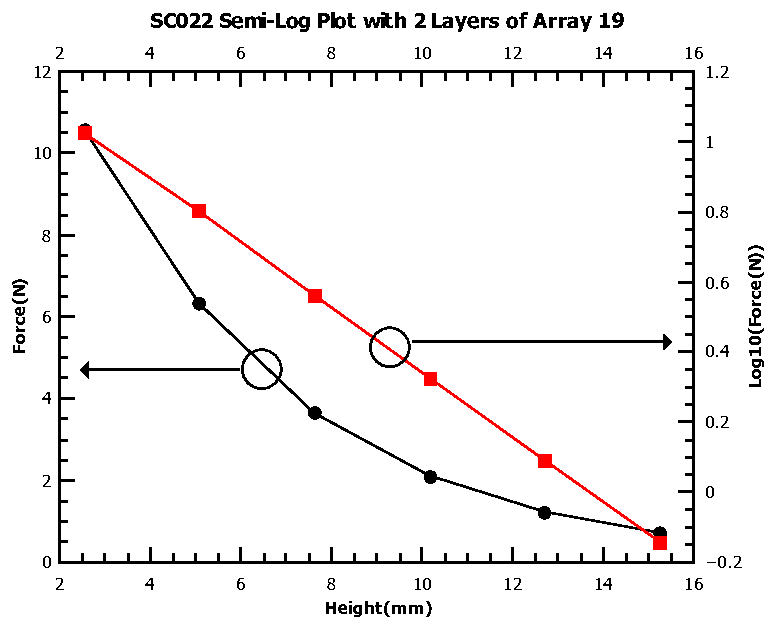
\includegraphics[width=3in]{SC022DoubleWith19.pdf}
\caption{Semi Log plot of the experimental force using SC022 and two layers of array 19 truncated at a maximum height of 15mm.}
\label{fig_force22_two}
\end{figure}

\begin{figure}[htbp]
\centering
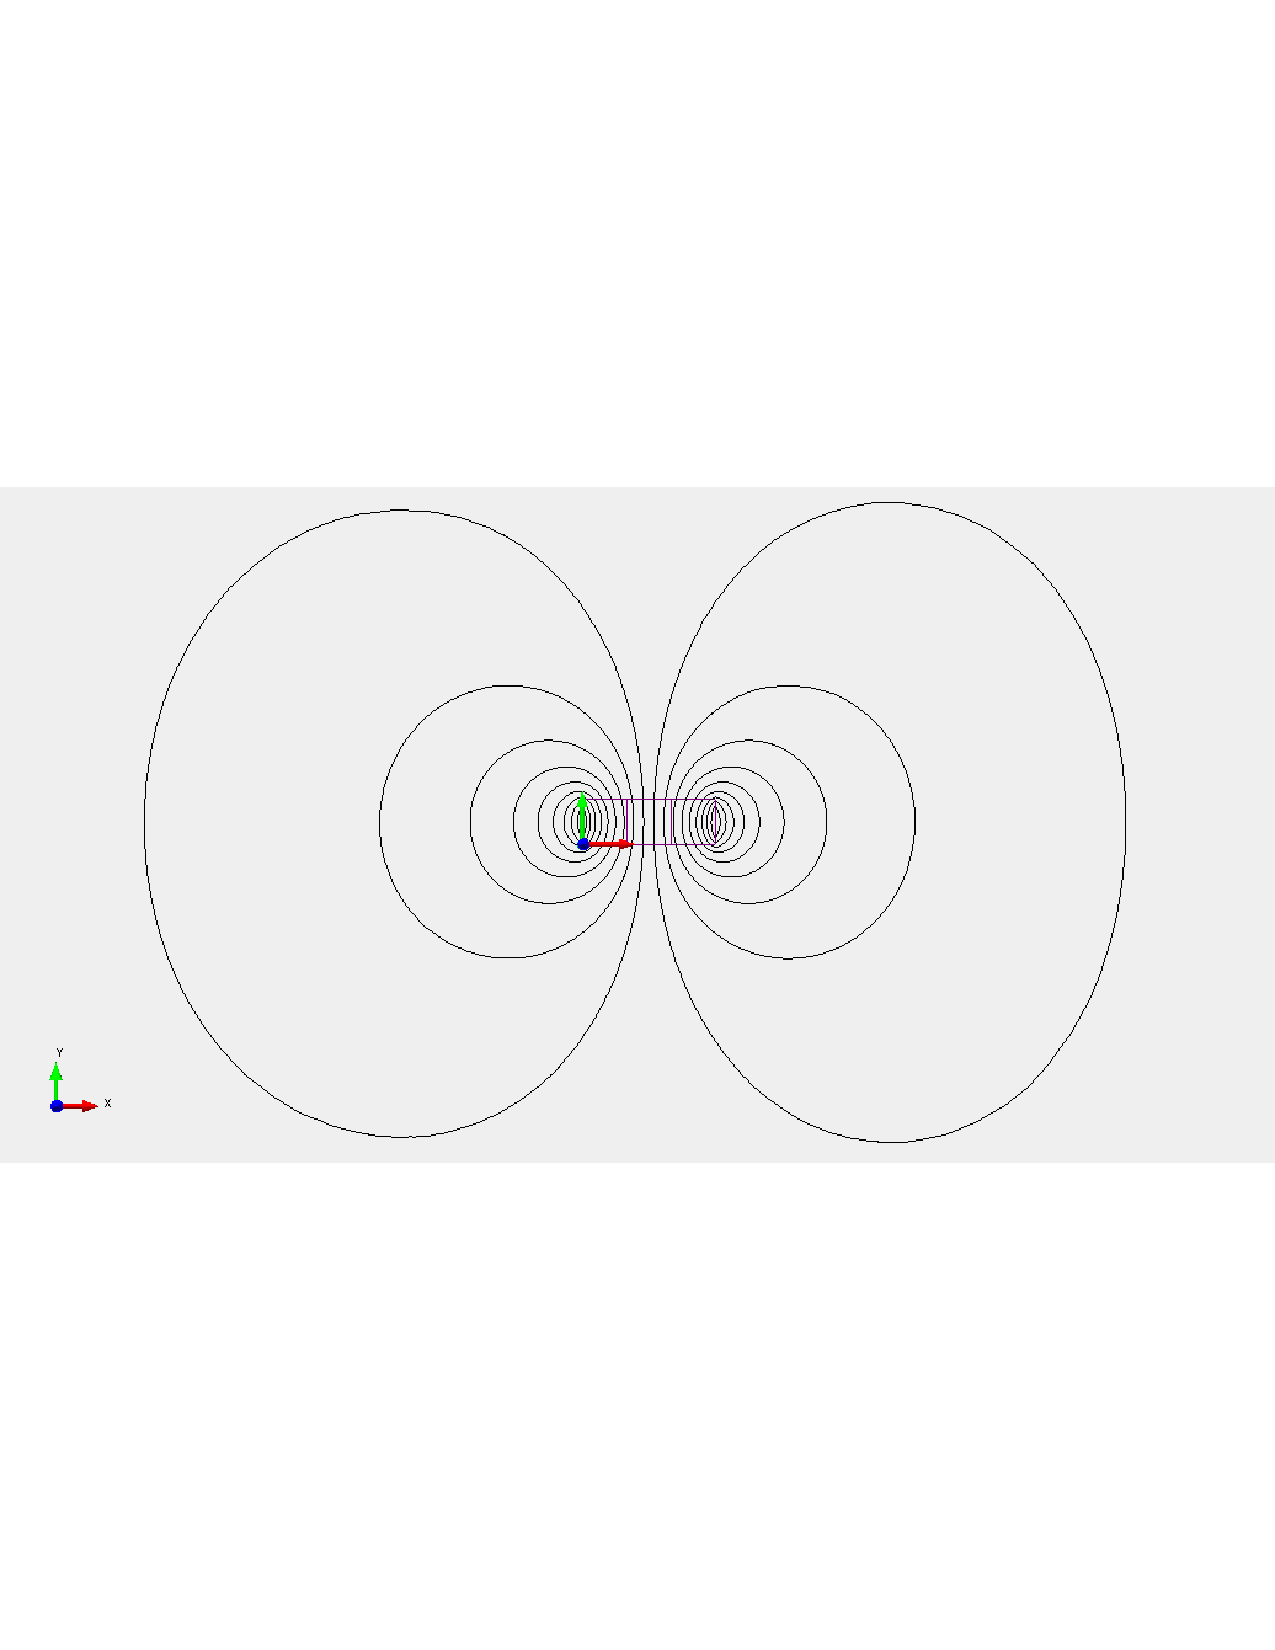
\includegraphics[scale=0.3, clip=true, trim=0cm 5cm 0cm 5cm\textwidth]{figures/FluxProfile1SingleLayer.pdf}
\caption{Flux profile of profile 1 in the orientation $\uparrow \uparrow \uparrow$.}
\label{fig_fluxprofile_1}
\end{figure}

\begin{figure}[htbp]
\centering
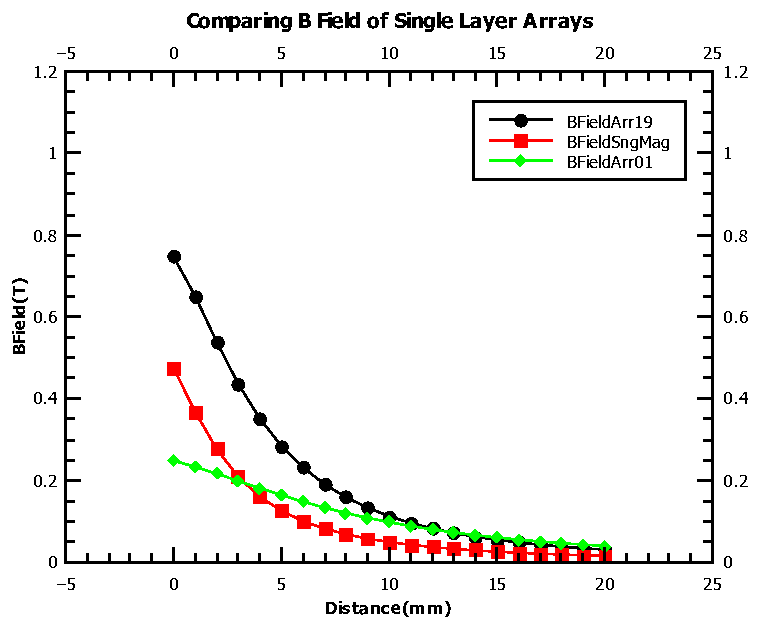
\includegraphics[width=3in]{BFieldSnLs.pdf}
\caption{Using FEA simulation data we compare the magnetic field between a single cube magnet, a single layer of profile 19 (three magnets in the orientation $\rightarrow\uparrow\leftarrow$) and a single layer of profile 1 (three magnets in the orientation $\uparrow\uparrow\uparrow$).}
\label{fig_BFieldSnLs}
\end{figure}

\begin{figure}[htbp]
\centering
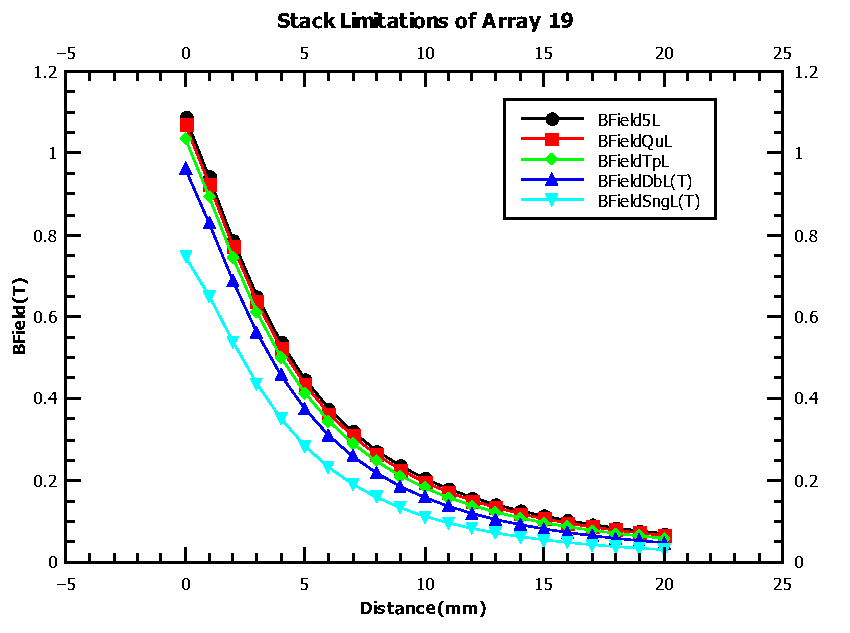
\includegraphics[width=3in]{StckLimArr19.pdf}
\caption{The simulation data shows a limitation in the increase of the B-field as a function of height from adding additional layers of profile 19.  The increase  drops off quickly after 3 layers.}
\label{fig_StckLimArr19}
\end{figure}

\begin{figure}[htbp]
\centering
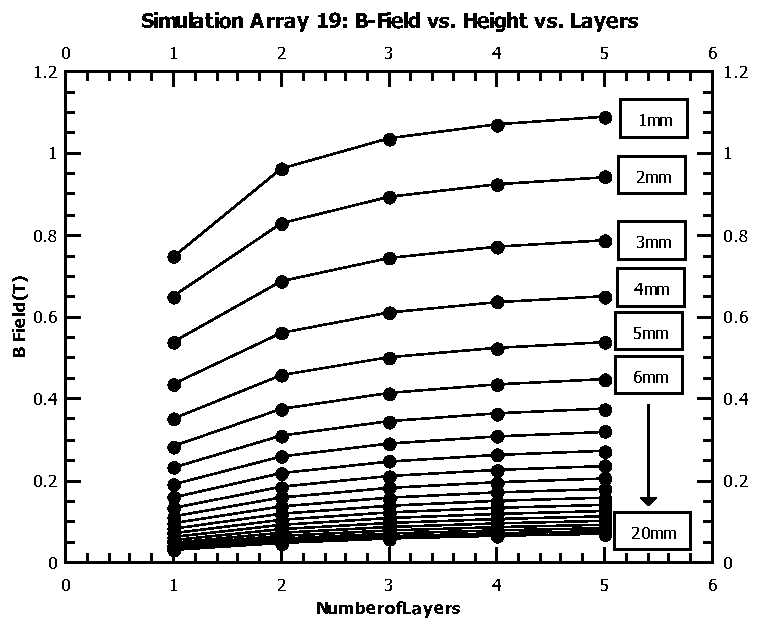
\includegraphics[width=3in]{BFieldVsLayerArr19.pdf}
\caption{Simulation data of the B-field from profile 19 as a function of the number of layers.  Each line represents an increase in the distance between superconductor and magnet array.}
\label{fig_BFieldVsLayerArr19}
\end{figure}

\begin{figure}[htbp]
\centering
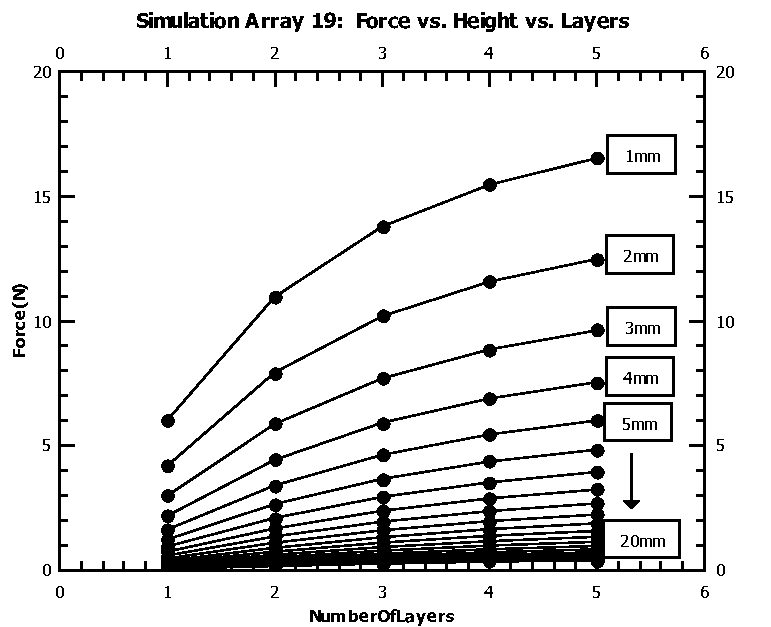
\includegraphics[width=3in]{FVsHVsLArr19.pdf}
\caption{Simulation data of the Force from profile 19 as a function of the number of layers.  Each line represents an increase in the distance between superconductor and magnet array.}
\label{fig_ForceVsLayerArr19}
\end{figure}

\begin{figure}[htbp]
\centering
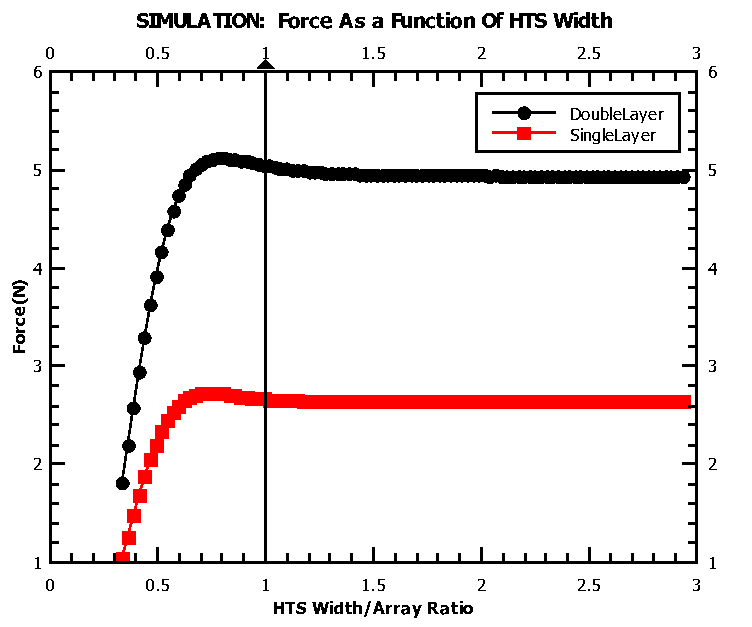
\includegraphics[width=3.3in]{ForceFncWidthArrOneAndTwoLyrs.pdf}
\caption{Simulation results of the force versus varying width of the HTS against profile 19.  The HTS maintained a height of 6.35mm but the width was slowly increased. }
\label{fig_ForceWidthArr19}
\end{figure}

\begin{figure}[htbp]
\centering
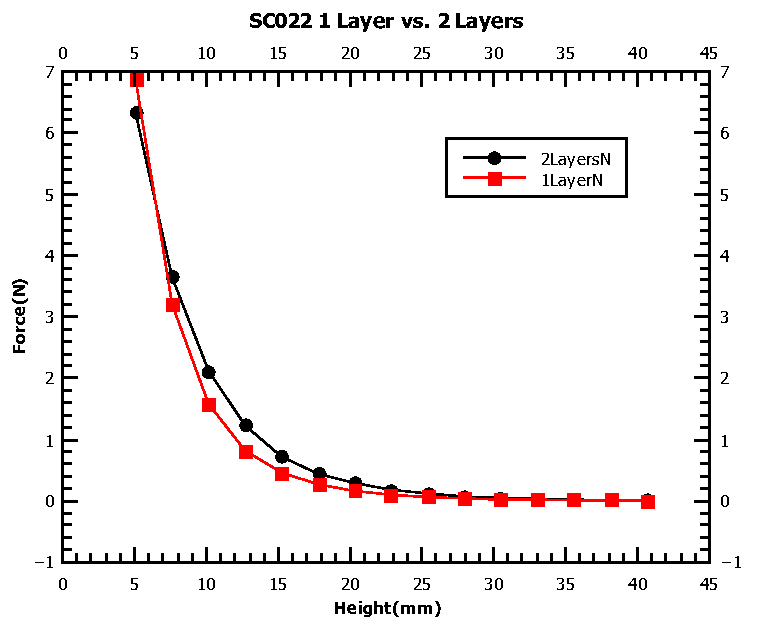
\includegraphics[width=3in]{figures/SC0221LayerVs2Layers.pdf}
\caption{Experimental result of the force on a HTS with 1 and 2 layers of profile 19. There is no significant increase at 5-7mm.}
\label{fig_1layervs2}
\end{figure}

\begin{figure}[htbp]
\centering
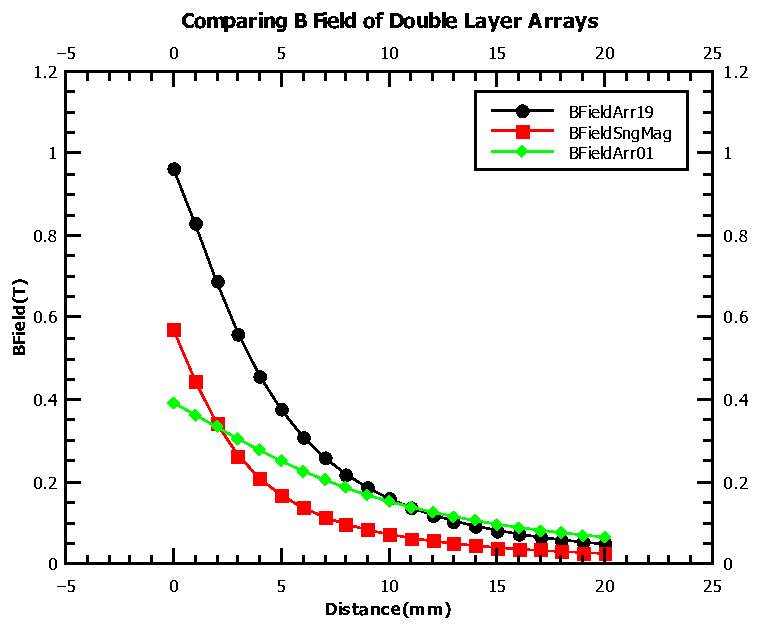
\includegraphics[width=3in]{BFieldDbLs.pdf}
\caption{Using FEA simulation data we compare the magnetic field between two stacked cube magnets, a double layer of profile 19 (three magnets in the orientation $\rightarrow\uparrow\leftarrow$) and a double layer of profile 1 (three magnets in the orientation $\uparrow\uparrow\uparrow$).}
\label{fig_BFiledDbLs}
\end{figure}

%%%%%%%%%%%%%%%%
% Chapter 4
%%%%%%%%%%%%%%%%

\chapter{The Effect of Ebola Glycoprotein Evolution on Protein Flexibility}
CA Mirabzadeh

%\section*{Abstract}

\section{Introduction}

The 2014 Ebola epidemic has provided a wealth of information that can be used to understand Ebola evolution and how it could modify the efficacy of vaccines. The goal of this study is to determine the effects of previous, ongoing, and future viral evolution on the structure and antibody binding properties of Ebola glycoprotein (GP). Our focus is on the disordered mucin-like domain of GP. Analysis suggests that, while most of the disordered region of GP is evolving in a neutral fashion \cite{Olabode2015, Li2014}, a few sites are undergoing positive selection, FIG. \ref{ebolagp}.

\section{Methods}
Molecular dynamics simulations were performed using the GROMACS \cite{Berendsen1995} simulation package. Neutral capping was used to ensure there were no electrostatic interactions between the ends of the peptides. Simulated tempering was used to increase the exploration of conformational space. Simulations were initiated with fully extended peptide conformations generated using the Python package PMX  \cite{Gapsys2015}.

\section{Results Discussion and Conclusion}

In order to understand selection relative to the flexibility of mutations we focused on positively selected sites, (Table \ref{possites}), in the disordered mucin-like domain of the Ebola virus glycoprotein.  We looked at flexibility, FIG. \ref{avgrms}, by averaging the root mean square deviation over five separate simulations of the disordered sites with positively selected peptides. In the future we would like to look at the entire mucin-like domain and see how multiple mutations work together to change flexibility.

\begin{table}[ht]
\caption{Positively selected sites. Three pairs of sequences from human sources used for our analysis. The first of each pair is a representative of a current sequence. The second simply has the ancestral amino acid inserted at the center position. The Democratic Republic of the Congo (DRC) is a country located in Central Africa. From 1971 to 1997 it was named Zaire.}
\centering
\begin{tabular}{ccc}
\hline \\
Residue & Sequence & Origin \\
\hline \\
L at 442 & SKGTDLLDPAT & Zaire 1995 \\
Ancestor at 442 & SKGTDFLDPAT & \\
S at 442 & SKSADSLDLAT & DRC 2014 \\
Ancestor at 442 & SKSADFLDLAT & \\
L at 429 & TAAGPLKAENT & Zaire 1995 \\
Ancestor at 429 & TAAGPPKAENT & \\
P at 376 & STSPQPPTTKT & DRC 2014 \\
Ancestor at 376 & STSPQSPTTKT &  \\
\hline \\
\end{tabular}
\label{possites}
\end{table}

\section{Acknowledgments}

Grant support for this research was provided by the National Science Foundation (DEB1521049) and the Center for Modeling Complex Interactions sponsored by the National Institutes of Health (P20 GM104420). Computer resources were provided in part by the Institute for Bioinformatics and Evolutionary Studies Computational Resources Core sponsored by the National Institutes of Health (P30 GM103324).


\begin{figure*}[htbp]
    \centering
    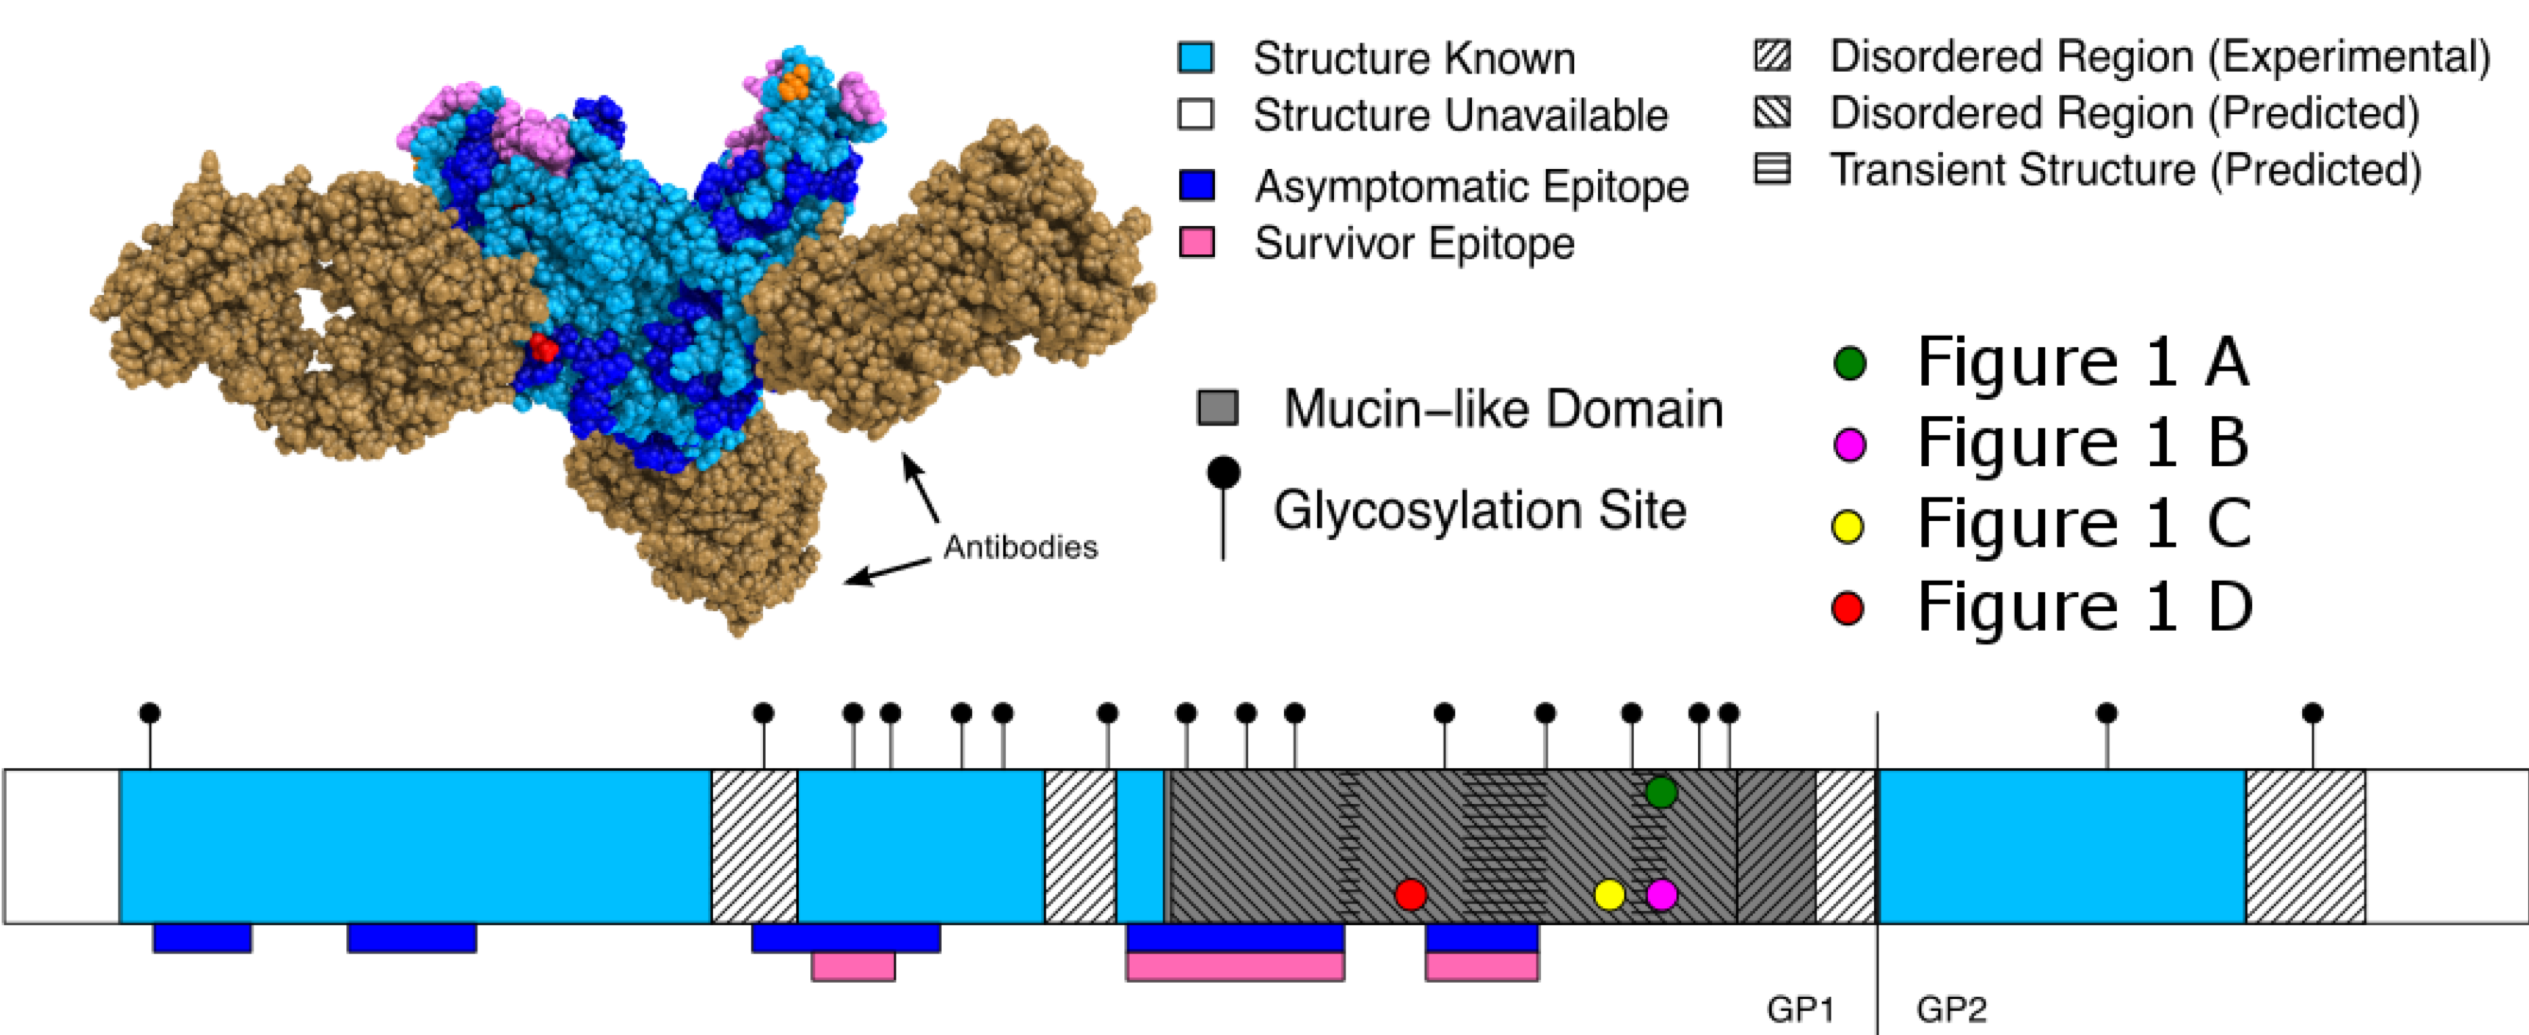
\includegraphics[width=1 \textwidth]{figures/ebolagraphic002.png}
    \caption{The Ebola glycoprotein. The positively selected sites are in the mucin-like domain. Evolutionary analysis results show that there has been some evolution that may change the way that antibodies bind to GP.}
    \label{ebolagp}
\end{figure*}

\begin{figure*}[htbp]
    \centering
    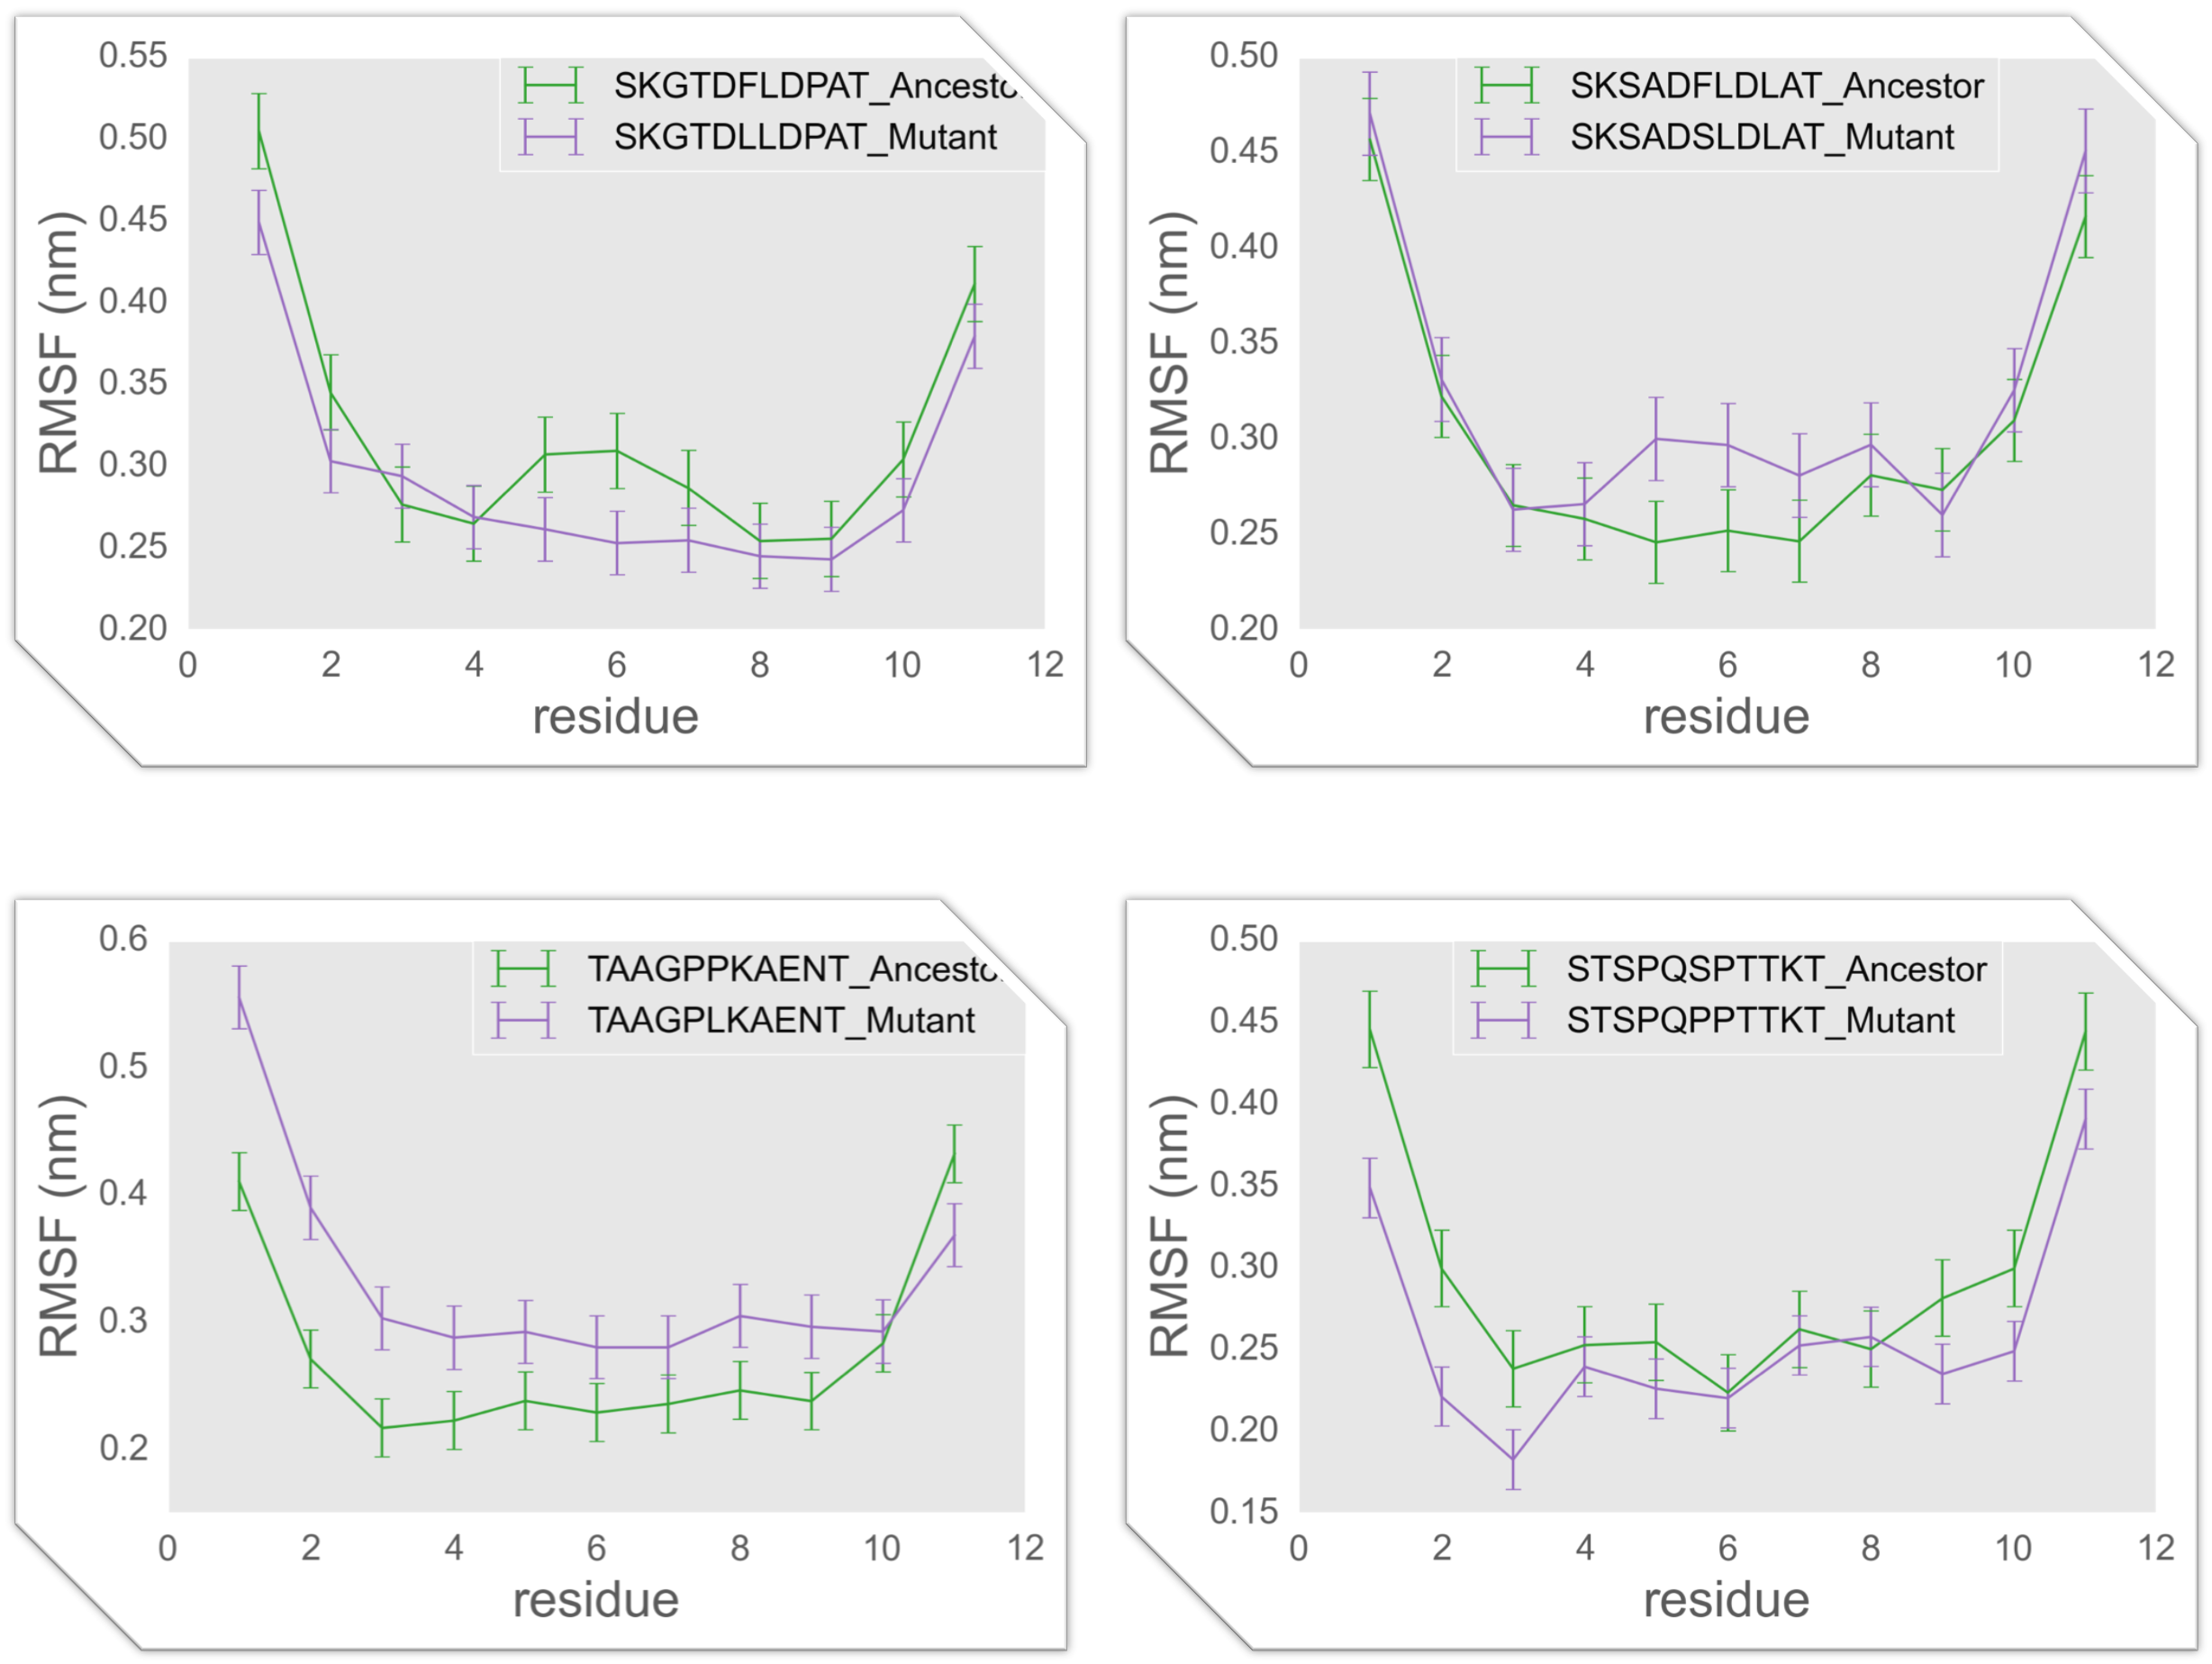
\includegraphics[width=1\textwidth]{figures/ebolagraphic001.png}
    \caption{Average C-alpha Root Mean Square Fluctuation. To understand the biophysical implications of mutations in the Ebola glycoprotein mucin-like domain, we performed molecular dynamics simulations of small fragments of the protein. The Root Mean Square Fluctuation was averaged over five separate time evolution simulations for each peptide.}
    \label{avgrms}
\end{figure*}

%%%%%%%%%%%%%%%%
% Conclusion
%%%%%%%%%%%%%%%%

%\clearpage
\section*{CONCLUSION}
\addcontentsline{toc}{chapter}{Conclusion}

Computational simulations allow us to explore "what if" situations by building a mathematical model which contains all of the parameters of the physical system in virtual form. In this way, costly, time-consuming or unsafe experiments may be avoided and performed "in-silica" cheaply and in a time efficient manner. The power of computational simulation is in the ability to facilitate the understanding of a system's behavior without actually testing the system in the real world. In addition, simulation can support experimentation where simulation represents systems or generates data needed to meet experiment objectives. 

Within the first part of this dissertation we showed a particular method, AIM, to be superior to the other methods in the context of what was tested. Further more, we found ways to improve the design of our simulation by showing that the density of intermediate states is directly related to the agreement between the methods, e.g. there must be sufficient sampling of the lambda states for convergence. In fixed lambda simulations the problem lies in the density of the chosen lambda states. Some states will contribute disproportionately to the variance of the estimate, therefore testing short simulations of different lambda densities before attempting longer simulations is a more economical use of time and resources. We found that running a longer simulation in a state space that is not dense enough to fully describe the state function propagates sampling error in regions of high variance. In contrast, lambda density should be increased in regions of high variance. By not increasing the density of states one is not able to achieve the required  ‘smoothness’ of the function in regions of high variation. This was a very important find for our future experiments where we will explore larger protein systems and more complex mutations.

For the second part of this dissertation we used 2D Finite Element Analysis in order to determine the optimal configuration for our permanent magnet arrays. These simulations allowed us to massively reduce the amount of work needed to perform our experiments. We were able to find the optimum configuration of magnets by programmatically exploring every possible configuration in a matter of hours instead of spending months in a lab. We note that the simulation is a simplification, i.e. a 2D Finite Element Analysis is limited in its ability to predict the interactions between magnetic flux penetration and High Temperature Superconductors. However, exploring every possible combination of permanent magnet arrays in the lab is nearly impossible. The simulations allowed us to reduce the costs of creating physical equipment to hold the magnets in place and expensive equipment to accurately measure the magnetic fields produced by the arrays. We stipulate that the simulation data is only appropriate for initial guess work and tells us very little of the underlying physics. In order to more accurately account for flux penetration and leakage, a 3-dimensional, non-linear solver is required. This would be something appropriate for future work in this study.

%%%%%%%%%%%%%%%%
% References
%%%%%%%%%%%%%%%%
\clearpage
\section*{REFERENCES}
\begin{singlespace}  % use single-line spacing for multi-line text within a single reference
	\setlength\bibitemsep{\baselineskip}  %manually set separataion betwen items in bibliography to double space
% 	\printbibliography[title={References}]
    \printbibliography[heading=none]
\end{singlespace}

\addcontentsline{toc}{chapter}{References}  %add References section to Table of Contents

%%%%%%%%%%%%%%%%
% Appendices
%%%%%%%%%%%%%%%%
\clearpage
%Appendix A

\section*{APPENDIX: USING AIM}

\addcontentsline{toc}{chapter}{Appendix: Using AIM}  %add Appendix section to Table of Contents

The GROMACS developers will have to review and accept the code changes that I have created. If the changes in the GROMACS code are accepted, the developers will maintain the code. Before they accept the changes they have to review it closely. They take on a majority of the responsibility. If not, then new releases break the code.

Simulations are set up as a standard expanded ensemble simulation with one modification. To use AIM set lmc-move = aim. The output of AIM will be in the log file of your simulation run.

The edited files are included in a github repository:\\ https://github.com/bioSandMan/gmx514.

Example expanded.mdp file:

\begin{lstlisting}
include                  = -I/mnt/ceph/cmira/pmxffs/mutff45
integrator               = md-vv
tinit                    = 0
dt                       = 0.001
nsteps                   = 10500000 ; 1 ns per lambda
comm-mode                = Linear
nstcomm                  = 1
nstlog                   = 10000
nstenergy                = 10000
nstlist                  = 20
ns_type                  = grid
pbc                      = xyz
rlist                    = 1.15
coulombtype              = Reaction-Field
coulomb-modifier         = Potential-shift-Verlet
rcoulomb                 = 0.9
cutoff-scheme            = Verlet
vdw-type                 = Cut-off
rvdw-switch              = 0.85
rvdw                     = 0.9
fourierspacing           = 0.12
pme_order                = 4
ewald_rtol               = 1e-04
ewald_geometry           = 3d
epsilon_surface          = 0
DispCorr                 = EnerPres
tc-grps                  = System
tcoupl                   = Nose-Hoover
tau_t                    = 0.1 ; can increase stability for
smaller ligands to have a low tau_t 
ref_t                    = 300
nsttcouple               = 1 ; can increase stability for
smaller ligands 
Pcoupl                   = no
tau_p                    = 5.0
compressibility          = 4.5e-5
ref_p                    = 1.01325
nstpcouple               = 1 ; can increase stability for
smaller ligands  
constraints              = all-bonds
constraint-algorithm     = shake    
;--------------------
; Free energy parameters
; Use expanded ensemble methods
free-energy              = expanded
sc-power                 = 1  
sc-r-power               = 6
sc-alpha                 = 0.5
init-lambda-state        = 0  
coul-lambdas             = 0.0 0.2 0.4 0.6 0.8 1.0 1.0
1.0 1.0 1.0 1.0 1.00 1.0 1.00 1.0 1.00 1.0 1.00 1.0 1.00
1.0
vdw-lambdas              = 0.0 0.0 0.0 0.0 0.0 0.0 0.1
0.2 0.3 0.4 0.5 0.55 0.6 0.65 0.7 0.75 0.8 0.85 0.9 0.95
1.0
nstdhdl                  = 1
nstexpanded              = 1
nstcalcenergy            = 1 
lmc-move                 = aim
separate-dhdl-file       = no
\end{lstlisting}

\end{document}
